\documentclass{projekt}
\usepackage[none]{hyphenat}
\usepackage{url}
\usepackage[utf8]{inputenc}
\usepackage[T1]{fontenc} 
\usepackage{ae}
\usepackage{fancyhdr}
\usepackage{graphicx}
\usepackage{pdfpages}
\usepackage[all]{xy}
\usepackage[czech]{babel}
\usepackage[activate={true,nocompatibility,all}, stretch=10, shrink=10, step=1, auto=true, draft=false]{microtype}
%\usepackage[total={17cm,28cm}, top=3cm, left=2cm, includefoot]{geometry}
\frenchspacing
\author{Filip Markvart}
\title{EEG/ERP portál}
\titlet{- transformace do sémantického webu} 
\titlett{}
\university{Západočeská univerzita v Plzni}
\faculty{Fakulta aplikovaných věd}
\department{Katedra informatiky a výpočetní techniky}
\subject{Bakalářská práce}
\town{Plzeň}
\begin{document}
\pagestyle{fancy}
\renewcommand{\chaptermark}[1]{\markboth{\textit{#1}}{}}
\renewcommand{\sectionmark}[1]{\markright{\textit{#1}}{}}
\cfoot{\thepage}
\lhead{\leftmark}
\rhead{\rightmark}
\maketitle
\chapter*{Prohlášení}
\thispagestyle{empty}
Prohlašuji, že jsem bakalářskou práci vypracoval samostatně a výhradně s~použitím citovaných pramenů.
\vskip 1.5em
V Plzni dne \today
\vskip 0.7em
\hskip 9cm Filip Markvart
\chapter*{Abstract}
\thispagestyle{empty}
\hspace{0.65cm}This thesis describes a transformation of neuroinformatics metadata stored in the relational database to the semantic web standard. The main goal is to investigate existing tools and necessary modifications that ensure automatic transformation for converting input data. The modified tool is able to process additional semantic information that cannot be stored in the relational database.


The last part describes design and implementation of an application that uses annotations to add semantic information to transformed data.

\tableofcontents
\pagestyle{fancy}
\renewcommand{\chaptermark}[1]{\markboth{\textit{#1}}{}}
\renewcommand{\sectionmark}[1]{\markright{\textit{#1}}{}}
\cfoot{\thepage}
\lhead{\leftmark}
\rhead{\rightmark}
\parskip 1em
\chapter{Úvod}
\hspace{0.65cm}Vyšetření elektrické aktivity mozku a evokovaných potenciálů patří mezi standardní metody neurologického výzkumu. Tato měření jsou prováděna také v laboratoři Katedry informatiky a výpočetní techniky Západočeské univerzity v Plzni. Všechna zde naměřená data jsou uchovávána v databázi webové aplikace označené jako EEG/ERP portál. Aby bylo možné získané údaje prezentovat na serveru NIF (Neuroscience Information Framework) \cite{dvacetTri}, je zapotřebí všechna data převádět do některého ze standardních formátů sémantického webu. 

Cílem této práce je prozkoumat možnosti reprezentace dat v prostředcích sémantického webu a vybrat z nich nejvhodnější formát pro reprezentaci dat získaných z EEG/ERP portálu. Práce se v další kapitole zabývá samotnou transformací dat z portálu do vybraného formátu, kterou se snaží následně co nejvíce zautomatizovat tak, aby vyžadovala minimální uživatelské zásahy. V této části je také popsán nástroj použitý při transformaci, který je dále modifikován tak, aby umožňoval dodávat transformovaným datům další sé-\\mantické informace prostřednictvím Java anotací.


Následující kapitola se věnuje návrhu a implementaci nástroje pro explicitní přidávání sémantických informací anotacemi. Jeho testovaní je pak popsáno \\v předposlední kapitole této práce.


\setcounter{page}{1}
\chapter{EEG/ERP portál}
\hspace{0.65cm}EEG/ERP portál je webová aplikace vytvářená pro Katedru informatiky a výpočetní techniky Západočeské univerzity v Plzni. Výzkumná skupina katedry se zabývá experimenty podle definovaných scénářů, při kterých měří evokované potenciály osobám, které jsou vystaveny specifikovaným vlivům. Při těchto experimentech se měří velké množství údajů, které je potřeba vhodně zaznamenávat tak, aby je bylo možné později jednoduše analyzovat \\a zpracovávat. Vzhledem k tomu, že samotná měření provádí větší počet osob, které se mohou sdružovat do skupin, je zapotřebí systému, který umožňuje přístup a práci s daty pro více uživatelů. Z tohoto důvodu byl vytvořen EEG/ERP portál, který umožňuje veškeré experimenty uchovávat.


Tato webová aplikace umožňuje všem registrovaným uživatelům vytvářet experimenty, vkládat naměřené hodnoty, vyhledávat vložená data vlastní či jiných uživatelů a údaje stahovat. Uživatelé, kteří provádějí experimenty, se mohou sdružovat do skupin a na portálu si vzájemně vyměňovat informace mezi sebou či s jinými skupinami. 
Aby ukládaná data z měření měla co nejlepší vypovídací hodnotu, je zapotřebí zaznamenávat nejen samotné naměřené přístrojové hodnoty, ale také přidružené údaje experimentu – tzv. metadata. Těchto údajů je velké množství a mezi základní patří metadata o experimentu, měřící a měřené osobě a také údaje o scénáři. 
Analýzou tabulek databáze bylo zjištěno, že mezi nejdůležitější uchovávaná metadata patří následující údaje \cite{diplomka}:

\textbf{Metadata o experimentu}
\begin {itemize}
\item měřící osoba
\item měřená osoba
\item použitý scénář
\item počasí
\item začátek měření
\item konec měření
\item teplota
\item případné poznámky
\end{itemize}

\textbf{Metadata o osobě}
\begin {itemize}
\item skupina
\item jméno
\item příjmení
\item pohlaví
\item datum narození
\item kontaktní údaje
\end{itemize}

\textbf{Metadata o scénáři}
\begin {itemize}
\item vlastník
\item výzkumná skupina
\item název
\item popis
\item soubor se samotným scénářem
\end{itemize}

\vspace{1cm}
Veškerá naměřená data i metadata jsou uchovávána v databázovém systé-\\mu Oracle. Portál s těmito daty pracuje a získává je objektově relačním mapováním (framework Hibernate). Celý portál běží jako webová aplikace napsaná v jazyce Java a využívá mimo již zmíněných technologií také frame-\\work Spring MVC, Spring Security a Spring Core.


Aby bylo možné EEG/ERP portál zaregistrovat do NIF (Neuroscience Information Framework), je nutné veškerá naměřená data poskytovat v jazy-\\cích sémantického webu. 
Vzhledem ke struktuře metadat, jejichž transformaci je třeba provést, a požadavkům NIF se jeví jako nejpříznivější cesta převod do standardního formátu OWL (Ontology Web Language), který je prostředkem sémantického webu.

\chapter{Sémantický web}
\hspace{0.65cm}V současné době je web tvořen obrovským množstvím informací v podobě webových stránek pocházejících od různých organizací, komunit či jednotlivců. Uživatelé k nim mohou snadno získávat přístup prostřednictvím URI (Uniform Resource Identifier) adresy, vyhledávačů nebo hypertextových odkazů \cite{dva}. Takováto podoba webu je sice poměrně jednoduchá, ale má své limity, protože v nepřeberném množství informací se lze snadno ztratit či jen sklouznout k irelevantním informacím. Následující příklad, který uvádí \cite{dva}, názorně ukazuje hlavní problém. Chceme-li na webu vyhledat dokumenty, jejichž autorem je Eric Miller, vyhledávače nám vrátí spoustu odkazů na stránky, týkající se osob tohoto jména, či jen obsahující daný výraz nebo jeho část, ale nezajistí vždy nalezení skutečně požadovaných informací. Problémem je skutečnost, že vyhledávací roboti a podobné nástroje pouze hledají výskyt zadaných údajů bez ohledu na jejich význam, který je často klíčový.


 Cílem sémantického webu je vyvíjet technologie, které by umožnily, aby stroje „rozuměly“ datům, se kterými pracují. Snahou sémantické webu ale není jen dostávat přesnější výsledky při vyhledávání informací, ale také získávat data z více různých zdrojů, porovnávat je a zpracovávat a díky tomu vytvářet informace nové. Aby bylo s daty možné takto pracovat, je nutné nepublikovat je jako samotné, ale přidružovat k nim přídavná data, která zachycují kontext, strukturu a obsah -  metadata \cite{dvacetDva}. U výše uvedeného příkladu by to znamenalo, že pokud budeme publikovat dokumenty vytvořené osobou jmenující se Eric Miller, specifikujeme toto jméno do metadat jako autora dokumentu. Tím se zajistí provázání konkrétní osoby s konkrétním dílem. Užitím metadat je pak možné s obsahem webu pracovat jako s relační databází a v důsledku toho se dotazovat na její obsah pomocí jazyků jako je SPARQL (Protocol and RDF Query Language).


Celou myšlenku sémantického webu poprvé publikoval v květnu roku 2001 v časopise Scientific American zakladatel současného webu Tim Berners Lee \cite{tri}.
Sémantický web vychází z několika základních principů, které je nutno uvést.


\begin {itemize}

\item \textbf{Vše je možné identifikovat prostřednictvím URI}\\

\hspace{0.65cm}Na veškeré objekty reálného světa jako jsou lidé, místa či jiné věci je možné se odkazovat v sémantickém webu identifikátory. Jakýkoliv tvůrce webu tak může vytvořit jedinečný identifikátor URI a říci, že označuje nějaký konkrétní objekt skutečného světa. 

\item \textbf{Odkazy mezi jednotlivými zdroji a zdroje samotné lze typovat}\\

\hspace{0.65cm}Současný web sestává ze zdrojů a odkazů. Zdroje jsou webové dokumenty určené pouze pro koncové osoby, a neobsahují tak žádná metadata popisující jejich účel či vztah k ostatním dokumentům. Cílový čtenář si tyto informace dokáže obvykle odvodit z obsahu, což ale počítačové systémy neumí, nebo je to pro ně příliš složité. Řešením je nevytvářet mezi dokumenty obyčejné odkazy, ale jednotlivé vztahy mezi objekty také popisovat. Jak je patrné ze schématu na obrázku 3.1, vazby mezi objekty lze popsat hodnotami jako např. „je autorem“, „závisí na“ nebo „je verzí“. Díky existenci typování jak zdrojů, tak vazeb, je pak možné kupříkladu vyjádřit, že nějaký zdroj je pouze verzí jiného zdroje.

\begin{figure}[htb]
\begin{center}
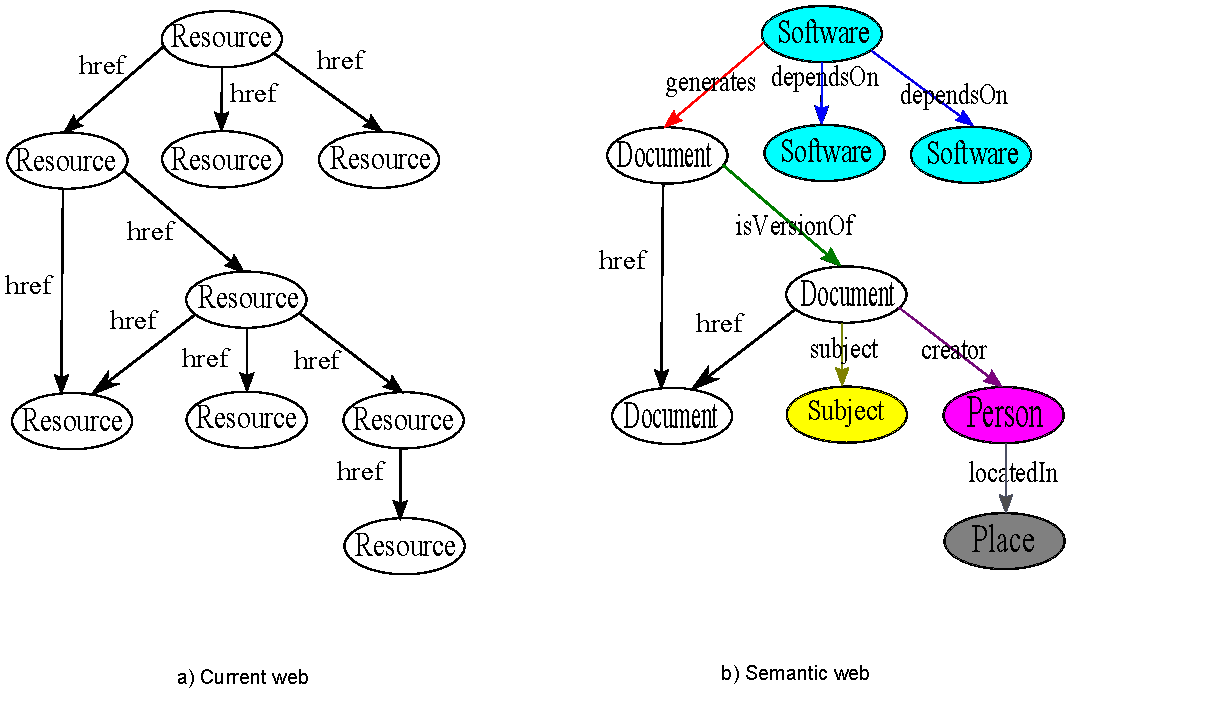
\includegraphics[scale=0.75]{Schema1.pdf}
\caption{Schéma provázání dat v současném a sémantickém webu \cite{dva}}
\end{center}
\end{figure}
\newpage
\item \textbf{Tolerance neúplných informací }\\

\hspace{0.65cm}Stejně jako u současné podoby webu, není nutné, aby odkaz zdroje byl neustále platný. Nedosažitelnost cílového zdroje tak není funkční překážkou, protože nástroje sémantického webu zpracovávají pouze dostupné informace, na základě kterých vytváří závěry. Stejně tak je možné zpracovávat jen vybrané úseky informací, ze kterých budou získávány neméně hodnotné výsledky. 

\item \textbf{Podpora paralelního vývoje dat}\\

\hspace{0.65cm}Zcela běžně může docházet k tomu, že různé skupiny osob vytváří obdobná data na různých místech nebo v jiném čase. Stejně tak se může u nich lišit použitá terminologie, ač skutečný význam obsahu je stejný. Díky prostředkům sémantického webu je možné např. s pomocí typovaných odkazů zajistit významovou provázanost obsahově obdob-\\ných či na sebe navazujících dat i když je forma jejich zápisu odlišná. Je tak možné přidávat nové informace, beze změny původních dat, na které se je stále možné odkazovat \cite{dva}.

\end{itemize}

\section{Architektura sémantického webu}
\hspace{0.65cm}Architektura sémantického webu je tvořena více vrstvami, které obsahují jednotlivé webové technologie a standardy.
Z obrázku 3.2 je celá architektura patrná. 
\begin{figure}[htb]
\begin{center}
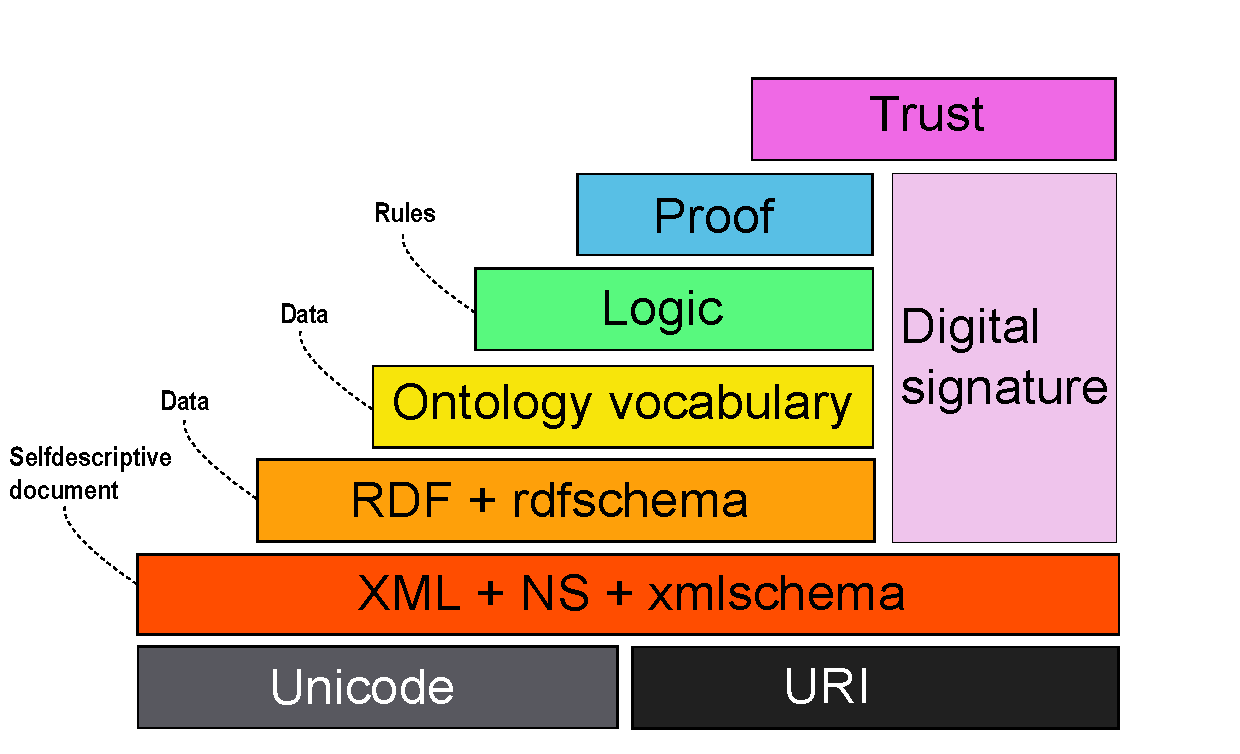
\includegraphics[scale=0.62]{architektura.pdf}
\caption{Architektura sémantickém webu \cite{dva}}
\end{center}
\end{figure}
Nejnižší vrstva určuje kódování mezinárodní znakovou sadou a jedno-\\značnou identifikaci objektů pomocí URI. Vrstva o úroveň výše zajišťuje definici dat pomocí XML (Extensible Markup Language) standardů. XML schéma zajišťuje strukturu XML dokumentů a zároveň XML rozšiřuje o da-\\tové typy.
Vrstva RDF + rdfschema popisuje strukturu metadat a zajišťuje typování zdrojů a odkazů. Poskytuje tím jednoduchou sémantiku pro datový model a díky RDF schématu i hierarchii zdrojů.


Vrstva ontologického slovníku zajišťuje přidávání ontologií a umožňuje tak konstruovat složitě vázané struktury díky obsahově rozšířenému slovníku pro popisování vlastností. Digitální podpisy pak umožňují detekci různých verzí dokumentů a jsou spolu se všemi předchozími částmi standardizované konsorciem W3C. Zbylé vyšší vrstvy standardizované nejsou a jsou neustále vyvíjeny.

\section{RDF}
\hspace{0.65cm}Technologickým základem celého sémantického webu je podle konsorcia W3C standard RDF(Resource Description Framework). Rámec RDF posky-\\tuje jednoduchý model pro popis zdrojů bez závislosti na jeho konkrétní implementaci \cite{tri}. Jedná se o jednoduchý jazyk, který umožňuje popisovat strukturu metadat tzv. trojicemi. Trojice je tvrzení, jež je tvořené subjektem, predikátem a objektem, které slouží k popisu zdroje. Pod touto trojicí je možné si představit tvrzení, že zdroj (subjekt) nabývá pro jistou vlastnost (predikát) nějakou hodnotu (objekt).


Subjektem může být libovolný objekt, který lze popsat identifikátorem URI, tedy např. webová stránka či předmět reálného světa.
Predikát je vlastnost, kterou má popisovaný subjekt. Objekt je pak hodnotou, které nabývá příslušný predikát a uceluje tak popis vlastnosti subjektu. Dle standar-\\du \cite{ctyri} je dokonce možné, aby objektem byl jiný subjekt (zdroj).
\newpage
Vzniklou trojící tak může být např. tvrzení: „Petr hraje tenis.“, jak je patrné z obrázku 3.3.

\begin{figure}[htb]
\begin{center}
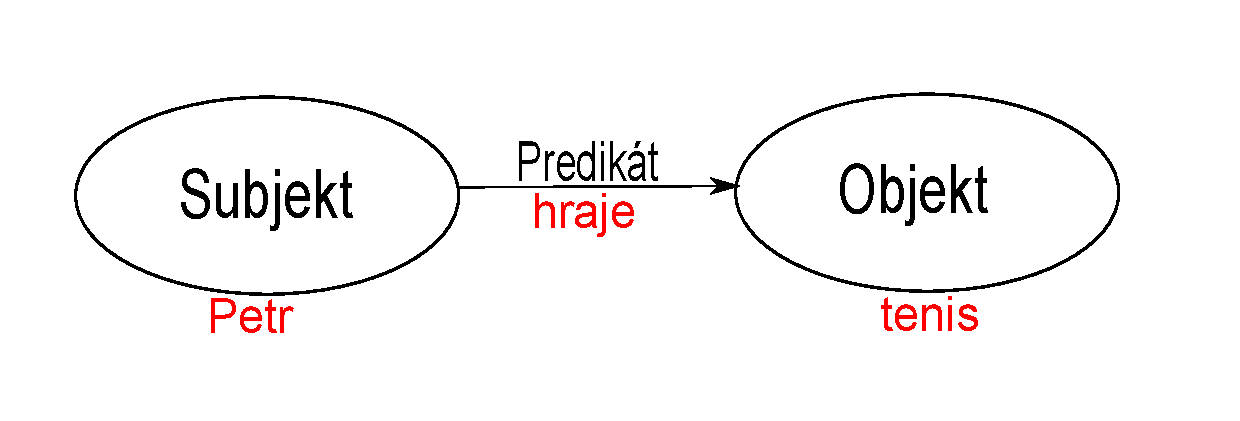
\includegraphics[scale=0.62]{trojice.pdf}
\caption{Příklad RDF trojice}
\end{center}
\end{figure}

Datový model RDF lze reprezentovat grafy nebo trojicemi, ale pro vyjádře-\\ní sémantiky webových zdrojů je nejvhodnější zápis syntaxí jazyka XML. Pomocí tohoto zápisu pak lze přiřazovat webovým zdrojům určité vlastnosti nebo mezi jednotlivými zdroji vyjadřovat vzájemné vztahy.
Příklad uvedený na obrázku 3.3., zapsaný standardizovanou syntaxí XML \cite{ctyri} vypadá násle-\\dovně.

\begin{verbatim}
<rdf:RDF xmlns:rdf="http://www.w3.org/1999/02/22-rdf-syntax-ns#"
         xmlns:dc="http://purl.org/dc/elements/1.1/">
  <rdf:Description rdf:about="http://www.w3.org/Person/Petr">
    <dc:hraje>tenis</dc:hraje>
  </rdf:Description>
</rdf:RDF>

\end{verbatim}


\section{Ontologie}

\hspace{0.65cm}Ontologie umožňuje vytváření metadat, tedy dodávání významových informací, které jsou klíčové v sémantickém webu \cite{sest}.
V informatice je ontolo-\\gie definována jako „formální specifikace sdílené konceptualizace“ \cite{pet}. Jedná se tedy o vytváření abstraktního modelu v určité oblasti – definování pojmů včetně jejich vzájemných vztahů, které jsou vyjádřené v logickém jazyce zpracovatelném počítačem. Veškeré pojmy tak musejí být explicitně specifiko-\\vány, aby informacím nerozuměli pouze lidé, ale i znalostně orientované systémy.\\
Ontologie se člení na 3 základní typy \cite{sest}:

\begin{description}
\item[Terminologické] - slouží především k získávání informací, nejvíce se blíží ke slovníkům synonym

\item[Informační] - slouží jako nadstavba databází a zajišťují kontrolu integrity a určitou abstrakci databáze potřebnou k dotazování

\item[Znalostní] - slouží pro reprezentaci znalostí v oblasti umělé inteligence 
\end{description}

Aby bylo možné ontologické informace formálně zapisovat, je zapotřebí jazyka, který by to umožňoval. Takových jazyků bylo vytvořeno poměrně velké množství a pro současnou podobu sémantického webu má největší význam OWL (Ontology Web Language).

\section{OWL}
\hspace{0.65cm}OWL je webový ontologický jazyk, který na rozdíl od předchozího RDF dovoluje vytvářet větší slovník a podrobnější syntaxi. Jeho vznik byl zapříčiněn potřebou získávat informace samotnými stroji (oproti současnému způsobu, kdy informace jsou získávány člověkem) \cite{sest}.
Oproti svému předchůdci má OWL širší vyjadřovací možnosti sémantiky, a tím zároveň i obsahu. 
Na rozdíl od jazyků RDF a RDFS (RDF Schema) umožňuje navíc definovat například:

\begin{itemize}
\item lokální omezení vlastností v rámci určité třídy, např. kardinalitu (sdílená nemovitost musí mít alespoň 2 vlastníky)
\item disjunktnost či ekvivalenci tříd, např. třída Vlastník je disjunktní se třídou Nemovitost
\item anonymní třídy (definované určitým logickým výrazem pro jednorázové použití)
\item matematické charakteristiky vlastností \cite{pet}
\end{itemize}

Jazyk OWL byl standardizovaný konsorciem W3C ve 3 variantách, které se liší se svou expresivitou.


\begin{itemize}
\item {\bf OWL Lite} je nejjednodušší verzí, která umožňuje definovat pouze hierarchii tříd a jednoduchá omezení.

\item {\bf OWL DL} je složitější variantou a zahrnuje veškeré konstrukce jazyka OWL, jejichž použití je ale omezené. Zkratka v názvu DL znamená, že tato verze využívá deskripční logiku.

\item {\bf OWL Full} je verzí, která zajišťuje maximální expresivitu. Umožňuje tak vytvářet velmi 
   složité konstrukce bez omezení předchozích verzí. 

\end{itemize}

Každá uvedená varianta je rozšířením verze svého předchůdce, který v ní může být plně vyjádřen \cite{sest}.\\
Co se týče možností syntaxe jazyka OWL, existuje dle specifikace W3C několik standardů, jejichž použití je patrné z tabulky 3.1.

\begin{table}[htbp!]

\label{značka tabulky}
\begin{center}
\begin{tabular}{|p{2.6cm}|p{10.0cm}|} 
\hline
RDF/XML &  Univerzální formát, který umožňuje migraci dat mezi různým softwarem\\
\hline
OWL/XML & Formát pro zpracování XML nástroji\\
\hline
Funcional Syntax & Formát vhodný pro zobrazení formální struktury ontologií\\
\hline
Manchester Syntax & Použití pro zápis a čtení DL verzí jazyka\\
\hline
Turtle & Užití pro tvorbu a získávání RDF trojic\\
\hline
\end{tabular}
\end{center}
\caption{Syntaxe jazyka OWL \cite{sedm}}
\end{table}

\chapter{Relační databáze a sémantický web}
\hspace{0.65cm}EEG/ERP Portál je webová aplikace běžící nad relační databází. Hlavním funkčním požadavkem, který by aplikaci umožnil registraci v rámci projektu NIF, je transformace ukládaných dat do prostředků sémantického webu. Transformace dat relační databáze je v zásadě možná dvěma způsoby \cite{diplomka}.

Prvním způsobem je provádět převod dat přímým přístupem k datům relační databáze. 
Z načítaných dat by se tak postupně vytvářely RDF struktu-\\ry, které by tvořily celý RDF graf.


Druhým způsobem transformace je přístup k datům databáze prostřednict-\\vím objektového datového modelu. Ten je možné snadno získat díky framewor-\\ku Hibernate \cite{osm}, který zajišťuje automatický a komplexní převod dat do POJO objektů (Plain Old Java Object). S využitím existujících nástrojů je pak možné manuální transformací získat data ve formátu RDF či OWL.

Hlavním problémem prvního způsobu transformace je ale skutečnost, že vytvářené RDF struktury nemají dostatečnou sémantiku, protože ji není možné z databáze získat. 
Možným řešením je dodávat sémantiku manuálním mapováním tabulek s předem vytvořenou ontologií. Nevýhoda tohoto přístupu nastává v situaci, kdy je zapotřebí změnit strukturu databáze. V takovém případě je pak nutné i ručně pozměnit způsob mapování.
Při transformaci druhým způsobem lze sémantiku dodávat přímo do objektového modelu. 
Datový model je možné snadno upravovat s využitím existujícího, dále popsa-\\ného nástroje, který dodává potřebnou sémantiku manuálně definovanými anotacemi.


Nástrojů, které provádí transformaci z relační databáze do jazyka RDF či sémanticky širšího OWL, několik existuje a jejich popis včetně zhodnocení je možné získat z \cite{diplomka}.
Z existujících nástrojů se pro potřeby portálu jeví jako nejvhodnější framework Jena, respektive Jenabean.



\section{Jena}

\hspace{0.65cm}Jena je framework, který slouží k vývoji aplikací sémantického webu. Tento nástroj je vyvinutý v jazyce Java jako open source. 
Framework v sobě obsahuje \cite{devet}:

\begin{itemize}
\item RDF API
\item OWL API
\item Dotazovací engine SPARQL
\item Možnost čtení a zápisu RDF dat ve formátu RDF/XML, N3 nebo N-triples
\item Ukládání RDF dat do databáze
\end{itemize}

Jena umožňuje snadnou práci s trojicemi a zajišťuje jejich ukládání do paměti ve dvou podobách \cite{diplomka}. První z možností je jednoduchý nízkoúrovňový graf, nad kterým jsou možné pouze základní operace pro vytváření nebo odebírání trojic a jejich vyhledávání.
Druhou možnou variantou uložení je vysokoúrovňový model, který nabízí daleko větší množinu možných operací nad daty. Nástroj obsahuje také tzv. Ontology API (Application Programming Interface), které umožňuje pracovat s ontologiemi, např. ve formátech RDF či OWL. Tyto ontologie se rovněž ukládají v podobě modelu, který nesestavuje nový graf, ale vytváří novou vrstvu nad původním modelem \cite{devet}.

Aby bylo možné tento nástroj využít k transformaci dat z relační databáze portálu do formátu sémantického webu, je zapotřebí tato data nejdříve získat a v požadované podobě je předávat ke zpracování. Díky frameworku Hibernate je možné data relační databáze převádět do objektového kódu ve formě POJO  objektů. Vzhledem k tomu, že samotná Jena takovýto vstupní formát přímo nepodporuje, je zapotřebí využít nadstavby označené jako Jenabean.

\section{Jenabean}   
\hspace{0.65cm}Jenabean je nástroj využívající API frameworku Jena sloužící ke tvorbě dat ve formátech sémantického webu \cite{deset}. Hlavním nedostatkem tohoto open source nástroje je, že kromě krátkého tutoriálu neobsahuje žádnou dokumen-\\taci. Jenabean umožňuje transformaci dat z objektově orientovaného kódu do ontologicky provázaných dat. Ta jsou vytvářena a uchovávána jako ontologický model Jeny. Díky této skutečnosti je možné vzniklý model uložit do souboru v podobě XML dokumentu. Nástroj rovněž podporuje opačnou transformaci dat – tedy z existujícího modelu Jeny do objektového kódu, a umožňuje i provádět SPARQL dotazy (prostřednictvím SPARQL enginu Jeny) nad vzniklým modelem. Pro účely této práce však postačuje využívat první způsob transformace.

Tento nástroj získává vstupní data z POJO objektů. Pro potřebu transfor-\\mace metadat z  Portálu do prostředků sémantického webu se jeví jako nejvhodnější formát OWL,  který dovoluje ukládat veškerou potřebnou séman-\\tiku a ontologie. K získání výsledného souboru ve formátu OWL je ještě nutné využít nástroj OWL API \cite{ctrnact}, který dokáže ze výstupního souboru generovaného z Jeny prostřednictvím Jenabeanu vytvořit OWL/XML soubor.

Veškeré klíčové ontologie určuje Jenabean primárně ze struktury objekto-\\vého kódu, tedy na základě příslušnosti jednotlivých atributů a metod ke třídám náležícím společným Java balíkům.
Ve struktuře sémantického webu jsou ontologie zapisovány užitím jmenných prostorů namespace, které tvoří prefix jednotlivých názvů entit. Takto vygenerované ontologie nemusejí vždy odpovídat skutečnosti a může být zapotřebí je upravit. Jenabean umožňuje nastavit implicitně jmenné prostory, které lze využít k určení ontologických vazeb transformovaných dat jako celku, takže veškeré entity pak budou náležet k definovanému jmennému prostoru. V případě potřeby detailnějšího určení ontologie entit mezi sebou navzájem pomocí jmenných prostorů i samotných názvů je možné jednotlivé POJO objekty rozšiřovat Java anotacemi.

\subsection{Použití nástroje Jenabean}
\hspace{0.65cm}API Jenabeanu poskytuje metody, díky kterým je možné provádět trans-\\formaci dat jednoduchým způsobem bez nutnosti podrobnějších znalostí práce s frameworkem Jena \cite{sedmnact}. 
V prvním kroku je nutné vytvořit prázdný model Jeny, který bude následně obsahovat veškerá zadávaná data. Jena nabízí dvě možné varianty modelu. Prvním je základní model ({\it Model}), který dovoluje uchovávat pouze jednoduché trojice v podobě RDF dat. Druhou variantou je ontologický model ({\it OntModel}), který rozšiřuje základní model o možnost dodávat datům další ontologie, jež lze využít v rámci jazyka OWL \cite{devet}. Tento model bude dále použit, protože dovoluje uchovávat ontologická data, která budou přidávána prostřednictvím Java anotatací nad POJO třídami, jak je uvedeno v následující kapitole.
Nad vytvořenou instancí modelu je pak možné provádět operace zápisu dat z POJO tříd prostřednictvím třídy {\it Bean2Rdf} a data zpětně z modelu načítat do objektové podoby užitím metod třídy {\it Rdf2Bean}. Nad instancí modelu je tedy možné pracovat prostřednictvím těchto tříd nebo lze využít zastřešující třídy {\it Jenabean} z Java balíku {\it thewebse-\\mantic.binding}, která po bindingu modelu poskytuje veškeré základní operace nad modelem. Finální zápis vytvořeného modelu do souboru ve formátu XML je možný prostřednictvím metody {\it write} nad instancí modelu nebo voláním metody {\it outFile} se String parametrem názvu výstupního souboru ze třídy {\it Bean2Rdf}, která byla doimplementována.  Následující příklad názorně ukazuje zápis dat POJO  objektů uložených v ArrayListu {\it objectList} do ontologického modelu a jeho následný export do souboru.

\begin{verbatim}
Model m = ModelFactory.createOntologyModel();

Jenabean.instance().bind(m);

// zápis jednotlivých POJO objektů do modelu
for (int i = 0; i < objectList.size(); i++) {
      Jenabean.instance().writer().save(objectList.get(i));
}
        
// exportování modelu do souboru
Jenabean.instance().writer().outFile("outputFile.xml");

\end{verbatim}


\section{Java anotace}
\hspace{0.65cm}Programovací jazyk Java umožňuje od verze 1.5.0 zapisovat do zdrojových kódů anotace. Anotace jsou formou metadat, která poskytují informace o pro-\\gramu, jež nejsou jeho přímou součástí \cite{jedenact}. Jedná se o zápis, který umožňuje přiřadit jednotlivým elementům ve zdrojovém kódu přídavné informace, aniž by byly přímou součástí kódu a mohly tak přímo ovlivňovat jeho činnost. Anotace mají široké spektrum užití, v zásadě lze ale rozlišit tři základní případy \cite{dvanact}.

\begin{itemize}
\item Dodání přídavných informací kompilátoru. Překladač může tyto infor-\\mace využívat k detekci chyb nebo potlačení varování.
\item Dodatečné informace pro zpracování dat při kompilaci. Některé softwa-\\rové nástroje využívají anotací jako dodatečných informací pro nasta-\\vení generování dalšího kódu, jako například při vytváření XML souborů.
\item Informace zpracovávané za běhu. Některé anotace je možné získávat\\ 
a využívat při běhu programu.
\end{itemize}

Zápis anotací se provádí při deklaraci tříd, metod, proměnných a dalších elementů programu. Anotace je možné používat jako samostatné – bez dalších uvedených parametrů, ale i s jedním nebo více. Příkladem první možnosti je {\it @override} anotace nad deklaracemi elementů překrývajícími elementy rodičovských tříd. Následující příklad ukazuje použití anotace v případě více elementů \cite{dvanact}.

\begin{verbatim}
@Author(
   name = "Benjamin Franklin",
   date = "3/27/2003"
)
class MyClass() { }
\end{verbatim}

Pokud by byl definován pouze jeden atribut s názvem „value“, není nutné uvádět jeho název a je možné využít jednoduššího zápisu níže:

\begin{verbatim}
@SuppressWarnings("unchecked")
void myMethod() { }
\end{verbatim}

Aby bylo možné vytvářet vlastní anotace, je nutné nejdříve vytvořit anotační typ. Jedná se 
v podstatě o definici rozhraní, kde je nutné před klíčové slovo interface uvést znak {\it @}.\\ 
Následující příklad ukazuje možné řešení \cite{dvanact}.

\begin{verbatim}
@interface ClassPreamble {
   String author();
   String date();
   int currentRevision() default 1;
   String lastModified() default "N/A";
   String lastModifiedBy() default "N/A";
}
\end{verbatim}

Deklarace jednotlivých metod anotačního rozhraní musí být bez parametrů a jejich návratové hodnoty jsou omezeny na primitivní datové typy, {\it String, Class, enum} a pole všech předchozích typů. Metodám lze také nastavit výchozí hodnoty, čehož lze využít, pokud se hodnota elementu v případě použití anotace mění jen zřídka. Pokud je hodnota elementu při anotaci explicitně zadána, musí se jednat o konstantu, která bude kompilátoru dostupná v čase překladu, v opačném příkladě je vyhozena výjimka. Při deklaraci anotačního rozhraní je také možné uvést takzvané meta anotace sloužící ke specifickému omezení použití anotace \cite{jedenact}.


První meta anotací je {\it @Retention}, která slouží k definici dostupnosti anotace. Jejím elementem může být \cite{trinact}:

\begin{itemize}
\item {\it RetentionPolicy.SOURCE} - dostupnost pouze ve zdrojovém kódu
\item {\it RetentionPolicy.CLASS} - dostupnost pro kompilátor
\item {\it RetentionPolicy.RUNTIME} - dostupnost virtuálnímu stroji za běhu programu
\end{itemize}


Druhou meta anotací je {\it @Target}, která svým elementem určuje omezení typů elementů, ke kterým může být anotace přidána. Těch existuje následu-\\jících 8 \cite{trinact}: 

\begin{itemize}
\item {\it ANNOTATION\_TYPE} - anotace pro anotace
\item {\it CONSTRUCTOR} - anotace konstruktoru
\item {\it FIELD} - anotace pole
\item {\it LOCAL\_VARIABLE} - anotace lokální proměnné
\item {\it METHOD} - anotace metody
\item {\it PACKAGE} - anotace Java balíku
\item {\it PARAMETER} - anotace parametru
\item {\it TYPE} - anotace třídy nebo rozhraní
\end{itemize}

Následující příklad deklarace rozhraní definuje anotace dostupné za běhu virtuálnímu stroji a použitelné k anotaci metod \cite{jedenact}.

\begin{verbatim}
@Retention(RetentionPolicy.RUNTIME)
@Target(ElementType.METHOD)
public @interface Test { }
\end{verbatim}

\section{Anotace nástroje Jenabean}
\hspace{0.65cm}Jenabean akceptuje 7 druhů možných anotací, kterými je možné obohatit požadovanou ontologii transformovaných dat \cite{deset}.

\begin{description}
\item[@Namespace] \indent anotace slouží ke změně implicitního jmenného prostoru pro celou třídu a zároveň se projeví u všech podřízených atributů a metod. Obsahuje jeden element  datového typu String nesoucí jméno jmenného prostoru. Cílem je správně ontologicky zařadit vytvořenou třídu do systému.
\item[@RdfType] je anotace sloužící ke změně implicitního názvu třídy na hodnotu definovanou v elementu datového typu String uvedené anotace. Název je přenesen i na ontologie podřízených atributů a metod. V případě užití samotné anotace {\it @RdfType} je v ontologii zachován implicitní jmenný prostor. Anotaci je možné použít zároveň v kombinaci s předchozím {\it @Namespace} za účelem změny názvu třídy i jmenného prostoru zároveň.

Z následující příkladu je patrný praktický zápis prvních dvou uvedených anotací \cite{deset}.

\begin{verbatim}
@Namespace("http://xmlns.com/foaf/0.1/")
@RdfType("Person")
public class Fellow {
        
        public String getName() {
                return name;
        }
        public void setName(String name) {
                this.name = name;
        }
}
\end{verbatim}

\item[@RdfProperty]anotace umožňuje společnou změnu jména i jmenného pro-\\storu jednoho atributu třídy pomocí jediné anotace. Slouží pro určení jednoznačné ontologické vazby, např. na jiného rodiče. Příklad možného zápisu \cite{deset}:\\

\begin{verbatim}

public class ExampleBean {

@RdfProperty
("http://semanticbible.org/ns/2006/NTNames#parentOf")
public Collection<Human> children;

}

\end{verbatim}

\item[@Id] je anotace, jež slouží k vygenerování unikátního klíče k atributům nebo metodám třídy, který je použit u názvu ontologie. Není vzájemně kombinovatelná s předchozí anotací. Jedná se o jedinou vyžadovanou anotaci, pokud není použita anotace {\it @RdfProperty}. Anotace nemá žádný element. Její použití je patrné z níže uvedeného příkladu \cite{deset}.

\begin{verbatim}
public class ExampleBean {
  
@Id
private int myid;

}

\end{verbatim}


\item[@Symmetric] anotace umožňuje nastavit elementu vlastnost {\it owl:Symmetric-\\Property}. Tato symetričnost v jazyce OWL znamená, že pokud dvojice prvků {\it (x,y)} je instancí symetrické třídy {\it T}, pak i dvojice prvků {\it (y,x)} je instancí třídy {\it T} \cite{patnact}. Prakticky to znamená, že pokud by například osoba A byla přítelem osoby B, pak je i osoba B přítelem osoby A.
Tuto anotaci je možné použít jak pro třídu, tak i pro její atributy.
Anotace nemá žádný atribut a její použití je tak analogické jako v případě anotace {\it @ID}.
\\

\item[@Transitive] je anotace, která cílovému elementu nastaví vlastnost {\it owl:Tran-\\sitiveProperty}. To znamená, že pokud dvojice prvků {\it (x,y)} je instancí tranzitivní třídy {\it T} a zároveň dvojice prvků {\it (y,z)} je také instancí třídy {\it T}, pak i dvojice prvků {\it (x,z)} je také instancí třídy {\it T} \cite{patnact}. Tuto vlastnost lze uvést na následujícím příkladu \cite{sestnact}:
Pokud třída savec je podtřídou třídy zvíře a zároveň zvíře je podtřídou třídy organismus, pak i savec je podtřídou třídy organismus.
Anotace je stejně jako v předchozím případě bez atributu a je ji možné využít pro třídu i její elementy.
\\
\item[@Inverse] anotace nastavuje vybranému elementu vlastnost {\it owl:InverseOf}. V jazyce OWL je možné objektům i vlastnostem přiřadit inverzní prvek. Použití lze demonstrovat na příkladu: Osoba vlastní auto. Vlastnosti {\it vlastní} je možné určit inverzní vlastnost {\it má majitele}, která je vlastností objektu {\it auto}. {\it @InverseOf} je zároveň symetrická, což ve výsledku usnad-\\ňuje hledání vztahů mezi jednotlivými objekty a vztah mezi objekty auta a osoba je tak jasně definován \cite{patnact}.

Tato anotace ale není funkční, a to ani v poslední verzi Jenabean 1.0.6. Vzhledem k této skutečnosti a faktu, že poslední verze nástroje byla uvolněna v únoru 2010, je nutné její opravu provést.\\
Nástroj obsahuje anotační rozhraní {\it Inverse}, které má jediný atribut sloužící k definici URI identifikátoru inverze cílového elementu. Použití této anotace se ale nijak ve výstupních datech neprojevuje. Nově navrže-\\ná a implementovaná úprava tedy zajišťuje načtení hodnoty atributu anotace a tato hodnota je pak zpracována a předána jako URI identifi-\\kátor hodnotě inverze cílového elementu, která je vytvořena pro přísluš-\\nou třídu či její atribut nesoucí tuto anotaci. Výsledné použití anotace je pak patné z níže uvedeného příkladu.

\begin{verbatim}
public class ExampleBean {

@Inverse
("http://semanticbible.org/ns/2006/NTNames#hasOwner")
public String hasCar;

}
\end{verbatim}
Výstup OWL API:
\begin{verbatim}
<InverseObjectProperties>
  <ObjectProperty IRI="http://www.kiv.zcu.cz/hasCar"/>
        <ObjectProperty IRI="http://semanticbible.org/ns/
         2006/NTNames#hasOwner"/>
</InverseObjectProperties>
\end{verbatim}


\end{description}




\section{Rozšíření nástroje Jenabean}
\hspace{0.65cm}Jazyk OWL dle své specifikace \cite{patnact} umožňuje dodávat datům více ontologií \\a sémantiky, než které nástroj Jenabean umí přidávat za použití Java anotací nad POJO třídami. 
Těchto možností jazyka OWL využívá framework Jena, který je schopen data obohatit o většinu sémantiky specifikovanou v jazyce OWL užitím prostředků svého OWL API. To je zároveň nutný předpoklad potřebný pro úpravu nástroje Jenabean tak, aby mohl užitím anotací také dodávat sémantiku transformovaným datům, protože tento nástroj sám nevy-\\tváří žádný vlastní model, ale pouze pracuje s ontologickým modelem Jeny.


Na základě těchto skutečností byl zadavatelem vytvořen seznam požado-\\vaných anotací, prostřednictvím kterých by mělo být možné dodávat datům požadovanou sémantiku v souladu se specifikací jazyka OWL. Názvy všech vytvořených anotací jsou zvolené tak, aby z nich bylo zřejmé, k jakým úpravám ve vzniklém OWL souboru bude jejich užitím docházet. 
Veškeré provedené úpravy nástroje jsou doprovázeny Javadoc komentáři popisujícími účel změn. To umožňuje jejich snadné vyhledání, neboť nástroj ve své původní verzi (až na několik výjimek) žádný Javadoc neobsahuje.\\


\begin{description}
\item[@DataRange] je anotace, umožňující nastavit omezení datového typu pro vybraný atribut třídy. Jazyk OWL poskytuje vlastnost {\it rdfs:range}, která slouží k omezení rozsahu dat.


OWL určuje datový typ referencí na existující XSD (XML Schema Datatype – schémový jazyk XML dokumentů) datové typy.  V případě použití restrikce více různými datovými typy je výsledek interpretován jako průnik rozsahů těchto typů \cite{patnact}. Definice vlastních datových typů, které by dovolovaly přesnější vymezení dat, jako například určení maxi-\\mální či minimální hodnoty, jsou ale možné až v jazyce OWL 2 \cite{sedmnact}. Nástroj OWL API, který provádí poslední krok transformace dat, sice tento jazyk podporuje, ale framework Jena nikoliv. Jena poskytuje prostřednictvím své třídy XSD datové restrikce na všechny primitivní datové typy XSD. Nástroj Jenabean je tak možné upravit, aby dovoloval přidání restrikce datového typu pro příslušný element, ale pouze referencí na existující XSD datový typ. XSD šablony dovolují vytvářet nové datové typy restrikcí či skládáním základních datových typů. Na tuto šablonu je pak sice možné při určení datového typu se odkázat, ale vzniká tím problém s přenositelností vzniklého OWL dokumentu, neboť je nutné vytvořenou šablonu buď zveřejnit nebo ji neustále přenášet spolu s dokumentem.

Vytvořená anotace tak má jeden atribut typu String, kterým se elementu určí restrikce buď na  primitivní datový typ XSD uvedením jeho názvu, nebo uživatelský typ URI identifikátorem adresy vytvořené XSD šablony. Při uvedení názvu XSD primitivního datového typu je nutné uvést jeho přesný název, s výjimkou typů {\it boolean, byte, double, float, int, long, short} a {\it String}, kde je nutné názvu předřadit prefix {\it x}, neboť se jedná o klíčová slova jazyka Java a implementace této anotace provádí dynamické čtení atributů tříd Jeny s příslušnými názvy. Například pro datový typ float je tak nutné uvést hodnotu {\it xfloat}.
Použití anotace je patrné z níže uvedeného příkladu.


\begin{verbatim}
public class Person {

@DataRange("nonNegativeInteger")
public int age;

}
\end{verbatim}
Výstup OWL API:
\begin{verbatim}
<DataPropertyRange>
  <DataProperty IRI="http://www.kiv.zcu.cz/age"/>
  <Datatype abbreviatedIRI="xsd:nonNegativeInteger"/>
</DataPropertyRange>

\end{verbatim}

\item[@VersionInfo] anotace dovoluje vybranému elementu přidat vlastnost {\it owl:-\\versionInfo}.
Jazyk OWL umožňuje přidávat objektům anotaci, která nese textovou informaci o verzi příslušného objektu. Jediný atribut typu String této anotace slouží k přímému zapsání informace. Nejedná se tedy o žádný URI identifikátor, jako v případě předchozích anotací. Každý objekt může nést pouze jednu informaci o své verzi, a proto při vícenásobném použití anotace bude uchována pouze poslední hodnota. Anotaci je možné využít pro třídu i její atributy, jak je patrné z následu-\\jícího příkladu.


\begin{verbatim}
public class Measuration {

@VersionInfo("Version 1.1")
private Scenario scenario;

}

\end{verbatim}
Výstup OWL API:
\begin{verbatim}
<AnnotationAssertion>
  <AnnotationProperty IRI="versionInfo"/>
  <IRI>http://www.kiv.zcu.cz/scenario</IRI>
  <Literal>Version 1.1</Literal>
</AnnotationAssertion>
\end{verbatim}




\end{description}


\chapter{Nástroj pro anotování POJO tříd}
\hspace{0.65cm}V předchozí kapitole byly popsané Java anotace nástroje Jenabean, jejichž užitím je možné obohacovat transformovaná data o další sémantiku, kterou není možné uchovávat v relační databázi z důvodu její nízké vyjadřovací schopnosti. Všechny tyto anotace musejí být zapisovány do POJO tříd, jež slouží jako persistentní objekty. Jejich zápis se provádí v místě deklarace samotných tříd, respektive jejich atributů, v závislosti na konkrétních typech anotace.
Tato skutečnost klade na uživatele požadavek ručně editovat jednotli-\\vé třídy, korektně zapsat příslušné anotace a následně  provést jejich překlad. Samotnou transformaci je tedy možné provést až po těchto krocích.


Vzhledem k tomu, že cílem této práce je požadovanou transformaci co nejvíce zautomatizovat tak, aby kladla na uživatele minimální nároky co se znalostí použitých nástrojů týče, je nutné zbavit ji požadavku na ruční editaci zdrojových kódů POJO.
Nejjednodušším řešením, které se intuitivně nabízí, by bylo načítání hodnot atributů anotací z externího souboru, jehož struktura by dovolovala snadné modifikace na jediném místě. Toto řešení ale není realizovatelné, neboť jazyk Java vyžaduje, aby hodnoty atributů anotací byly překladači známé již v době překladu, nikoliv až za běhu, kdy čtení externích souborů probíhá. Částečné řešení tohoto problému poskytuje nástroj Annotation File Utilities.

\section{Annotation File Utilities}

\hspace{0.65cm}Annotation File Utilities je open source nástroj vyvinutý v jazyce Java, který umožňuje přidávat anotace Java třídám \cite{osmnact}. Poslední uvolněná distribu-\\ce obsahuje skripty pro operační systém Windows i Linux sloužící k ovládání tohoto nástroje prostřednictvím příkazového interpretu. První skript s názvem {\it insert-annotations} provádí vložení anotací do přeložené třídy, jejíž název je uveden jako první parametr a druhým parametrem je soubor obsahující specifikaci vkládaných anotací. skript {\it insert-annotations-to-source} slouží ke stejnému účelu, ale anotace přidává přímo do nepřeloženého zdrojového souboru, který je opět uveden jako první parametr. Třetí a poslední skript {\it extract-annotations} extrahuje veškeré anotace přeložené třídy, jejíž název je uveden jako jediný parametr, do souboru shodného jména s příponou {\it .jaif}.
Soubor „jaif“ (Java anotation index file), který je vstupním parametrem prvních dvou skriptů, slouží k definici vkládaných anotací a určení jejich přesného umístění v cílové třídě. Z dodávané dokumentace včetně mnoha ukázkových příkladů je patrné, že nástroj je velmi komplexní a umožňuje vkládat jakékoliv anotace do libovolného místa třídy v souladu se syntaxí jazyka Java. Tato komplexnost s sebou ale zároveň přináší složitější zápis „jaif“ souboru, který musí mít v záhlaví uvedené definice všech použitých anotací. Ty představují analogii k anotačním rozhraním Javy, takže je nutné uvést název anotace, její atributy včetně datových typů a také dostupnost (pro kompilátor či virtuální stroj). 
Na dalších řádcích souboru se provádí zápis cesty k elementům, které mají být anotovány, tedy název Java balíku, třídy a případně cílové metody či atributu. Posledním údajem je pak název samotné anotace včetně uvedení hodnot atributů (pokud nějaké má).


Jeden „jaif“ soubor tak může obsahovat definice vkládaných anotací pro více tříd, což by umožňovalo anotovat POJO třídy úpravou jediného souboru, ale stále je nutné opakovaně spouštět patřičný skript pro každou třídu a uži-\\vatel by také musel být obeznámen se syntaxí „jaif“ souboru, která není zcela triviální, jak je patrné z níže uvedeného příkladu.

\begin{verbatim}
package thewebsemantic:

annotation @RdfProperty: 
@Retention(value=RUNTIME) 
@java.lang.annotation.Target(value={TYPE_USE})
String value

package data.pojo:
class Person:
field surname: 
@thewebsemantic.RdfProperty("http://www.kiv.zcu.cz/prijmeni")

\end{verbatim}

Výše uvedený příklad ukazuje přidání anotace {\it RdfProperty} (včetně para-\\metru) atributu {\it surname} třídy {\it Person}. 
Všechny tři skripty ve svém kódu volají knihovnu {\it annotation-file-utilities.jar}, která provádí samotnou operaci, a skripty jí předávají potřebné parametry. Díky této skutečnosti se otevírá možnost navržení programu, který by využíval zmíněnou knihovnu k anotování POJO tříd takovým způsobem, že by na základě požadavků uživatele přidával anotace akceptované nástrojem Jenabean vybraným třídám. Jenabean akcep-\\tuje pouze konečné množství anotací nad atributy a třídami, které by nástroj znal a uživatel by z nich pouze vybral ty, které požaduje, zvolil cílový atribut a třídu a nástroj by vygeneroval potřebný „jaif“ soubor a prostřednictvím zmíněné knihovny anotace dodal.
Realizaci toho nástroje popisuje následující podkapitola.

\section{Annotation tool}
\hspace{0.65cm}Cílem navrhnutého a následně implementovaného nástroje je zajištění jednoduchého dodávání anotací již přeloženým POJO třídám s minimálními nároky na uživatelovy znalosti dané problematiky. Nástroj musí nabídnou seznam všech dostupných anotací, které Jenabean dokáže zpracovat, z nichž uživatel požadované vybere a rozhodne o jejich umístění. Seznam dostupných anotací musí být modifikovatelný, tak aby umožnil přidávat další nové anotace pro případ rozšíření Jenabeanu o schopnost zpracovávat další anotace. Vybra-\\nou konfiguraci anotací je také nutné ukládat, tak aby bylo možné ji později jednoduše upravit. Pro zajištění jednoduchého ovládání je potřeba vytvořit grafické uživatelské rozhraní, které bude celý nástroj řídit.


\subsection{Analýza problému}
\hspace{0.65cm}Celý nástroj pracuje s přeloženými POJO třídami, které je nutné nejprve do aplikace načíst. Vzhledem k tomu, že upravovaných tříd může být větší počet, je zapotřebí umožnit jejich načítání v podobě jak jednotlivých souborů, tak i JAR (Java Archive \cite{devatenact}) souboru, ve kterém budou všechny třídy zabaleny. Protože JAR soubor, který primárně slouží jako snadno distribuova-\\telný archiv tříd pro vytvářené Java aplikace, je pouze adresář komprimovaný ve formátu ZIP, je možné využít standardní knihovny Javy k jeho extrakci. Všechny načítané POJO třídy je pak nutné zkopírovat respektive extrahovat z JAR archivu do pracovního adresáře aplikace, aby další operace nad těmito soubory mohly být jednotné. V dalším kroku je potřeba určit seznam názvů atributů jednotlivých tříd, neboť především ty budou anotovány. Názvy samotných tříd je možné převzít z názvů souborů, neboť dle specifikace Javy se musejí shodovat s názvy odpovídajících souborů. Seznam atributů je možné získat využitím Java Reflection API \cite{dvacetJedna} (dále jen reflexe), které umožňuje načítat třídy za běhu aplikace a získávat pak o nich detailní informace. Poslední data, která jsou nezbytná pro funkčnost nástroje, tvoří seznam přípustných anotací. Ten je potřeba rozdělit na dvě části – anotace pro třídy a pro jejich atributy. Seznamy budou načítány ze dvou textových souborů, respektující toto rozdělení. Ty ponesou pouze seznam názvů anotací včetně příznaků zda, mají parametr. Tím se docílí jednoduché modifikovatelnosti seznamu dostupných anotací.


Aby bylo možné se všemi načtenými daty efektivně pracovat, je zapotřebí vytvořit datovou vrstvu, která bude všechna data uchovávat. Ta bude mít hierarchickou strukturu, stejně jako elementy Java třídy, což zajistí dostateč-\\nou přehlednost uchovávaných dat. Pro každou načtenou třídu pomocí reflexe získáme seznam atributů. Každému z nich pak přiřadíme seznam dostupných anotací (získaný z výše zmíněného souboru). Totéž se učiní i pro samotné třídy. Jednotlivé anotace ponesou své jméno, příznak zda má být k příslušnému atributu či třídě přiřazena a hodnotu anotačního parametru (pokud jej má). Všechna data pak budou zabalena do jednoho objektu, který ponese seznam tříd, které budou obsahovat seznam svých anotací a atributů, které rovněž ponesou svůj seznam anotací.


Poté, co uživatel vybere a nastaví požadované anotace, je zapotřebí provést jejich zápis do příslušných POJO souborů. Ty jsou uložené v pracovním adresáři aplikace a jsou jedním ze vstupů knihovny {\it annotation-file-utilities.jar}, jež bude samotný zápis provádět. Druhým nutným vstupem je „jaif“ soubor, který je potřeba na základě požadovaných anotací vygenerovat. V prvním kroku se musí získat z datové vrstvy seznam všech přidávaných anotací, a to v takovém formátu, aby z nich bylo možné jednoduchým sekvenčním čtením generovat „jaif“ soubor. Musí tedy obsahovat kromě svého názvu a případné \\hodnoty i cílovou třídu a atribut (pokud nejde o anotaci třídy), kam má být zapsána, což lze snadno určit díky hierarchii dat. Z tohoto seznamu se pak získá další seznam všech neopakujících se názvů anotací (včetně informace, zda mají parametr), který bude použit pro vygenerování hlavičky „jaif“ souboru, jež nese definice přidávaných anotací. Tuto hlavičku lze jednoduše sestavit, protože jednotlivé anotace se liší pouze svými názvy a přítomností parametru, který je vždy typu String, a zbylé části lze považovat za konstantní řetězce. Samotný zápis cílů konkrétních anotací a případných hodnot se pak provede sekvenčním načtením všech potřebných dat ze seznamu přidávaných anotací a jejich vložením mezi klíčová slova „jaif“ souboru, které lze opět chápat jako konstantní řetězce. Po sestavení obsahu „jaif“ souboru se provede následné volání hlavní metody anotační knihovny, a to opakovaně pro každou modifikovanou třídu, přičemž v každé iteraci bude její název uveden jako parametr. Jako poslední krok je zapotřebí zkopírovat všechny třídy (včetně neanotovaných) do uživatelem zadaného umístění, čímž je dosažen požadovaný výstup tohoto nástroje.\\
Vzhledem k tomu, že anotační knihovna umí provádět pouze zápis anotací do souborů, ale neumožňuje již jejich modifikace a odstraňování, je nutné před jejím prvním voláním původní POJO soubory zkopírovat do dalšího adresáře, který poslouží k uchování jejich původní podoby. Z něj budou vždy před samotným zápisem anotací tyto soubory zkopírovány do pracovního adresáře, kde budou anotovány. Tím se docílí, že výsledné POJO třídy budou obsahovat právě ty anotace, které uživatel vybral a žádné jiné (přidané již dříve).


Aby bylo možné po ukončení aplikace a jejím opětovném spuštění navázat na provedené úpravy anotací, případně je měnit, je nutné ukládat na disk všechny tyto údaje. Zároveň může vzniknout požadavek na úpravu jiné sady tříd, přičemž provedené změny na předchozích třídách je také potřeba zachovat. Nejjednodušším řešením celého problému je ukládat všechna data – tedy upravované POJO třídy a uživatelem nastavené anotace na disk zabalené do jednoho souboru jako projekt. Ten by pak bylo možné opětovně načíst a pokračovat v  započatých změnách. Aby nedocházelo k ukládání redundantních dat, bude se vytvářet soubor, který ponese jen uživatelem vybrané a nastavené anotace včetně jejich cílového umístění, neboť ostatní data je možné opětovně získat reflexí. Soubor se vytvoří na základě seznamu přidávaných anotací, získaného stejným způsobem jako při generování „jaif“ souboru. Tento soubor se spolu se všemi POJO třídami z pracovního adresáře aplikace a soubory obsahujícími seznam přípustných anotací zabalí do ZIP archivu a uloží jako projekt na disk pod uživatelem definovaným jménem.


Posledním problémem, který je zapotřebí vyřešit, je otevírání uložených projektů. To bude probíhat analogicky jako načítání dat z JAR archivu při vytváření nového projektu s tím rozdílem, že je ještě potřeba načíst uložené změny (vybrané anotace). Po rozbalení archivu se všemi soubory do pracovního adresáře aplikace a načtení všech základních dat je nutné načíst soubor s uloženými anotacemi. Sekvenčním čtením se pak pro každou anotaci najde v datové vrstvě příslušná třída případně atribut a anotace se upraví na požadovanou hodnotu. Uložené soubory seznamů dostupných anotací pro třídy a atributy budou sloužit jako ochrana proti nekonzistenci dat v případě, že by se v uloženém projektu vyskytovaly anotace, které budou následně v seznamu těch základních, programu dostupných odstraněny. Při otevírání projektu se tak při získávání seznamu dostupných anotací budou načítat jak soubory určené pro samotnou aplikaci, tak i ty uložené v projektu. Ze všech získaných anotací se vytvoří jejich sjednocení, které bude tvořit nový seznam dostupných anotací pro aktuální projekt. Díky tomu bude možné ve starém projektu používat jak původní anotace, tak i nově přidané. 




\subsection{Popis implementace}
\hspace{0.65cm}Vytvořený nástroj je koncipován jako třívrstvá architektura, což je patrné ze struktury Java balíků.
Veškerá zpracovávaná data jsou uchovávána a zpří-\\stupňována prostřednictvím třídy {\it Project}. Ta nese list tříd {\it ClassItem}, jejichž jednotlivé instance představují jednu POJO třídu, která je anotována. Zde je uloženo jméno třídy, dále cesta k fyzickému souboru (potřebná k pozdější modifikaci) a listy tříd {\it Annotation} a {\it Attribute}. Třída {\it Annotation} reprezentuje jednu konkrétní anotaci, která je vázána na určitý element, tedy třídu nebo její atribut. Obsahuje název anotace, příznak, zda má být přidána a zadanou hodnotu atributu – pokud se jedná a parametrickou anotaci. V případě neparametrické anotace (což je rozlišeno dvoustavovou proměnnou) je tato hodnota prázdná. Třída {\it Attribute} pak reprezentuje jeden atribut POJO třídy, přičemž nese jeho název a list přítomných anotací reprezentovaných opět třídou {\it Annotation}. 
Datová vrstva obsahuje ještě abstraktní třídu {\it FileSaved-\\Annotation} a její dva potomky rozlišující, zda se jedná o anotaci atributu nebo třídy. Ty slouží k předávání jednotlivých anotací částem aplikace, které generují soubor „jaif“ a ukládají uživatelem vybrané konfigurace anotací jednotlivých tříd při ukládání projektu. Tato třída obsahuje, na rozdíl od třídy {\it Annotation}, všechny informace potřebné k zápisu anotace do „jaif“ souboru, tedy jméno třídy, atributu (pokud se jedná o anotaci atributu), ano-\\tace a její hodnotu, která je opět prázdná v případě neparametrické anotace. Celá struktura datové vrsty je patrná z UML diagramu na obrázku 5.1.
\vspace{1.0cm}

\begin{figure}[htb!]
\begin{center}
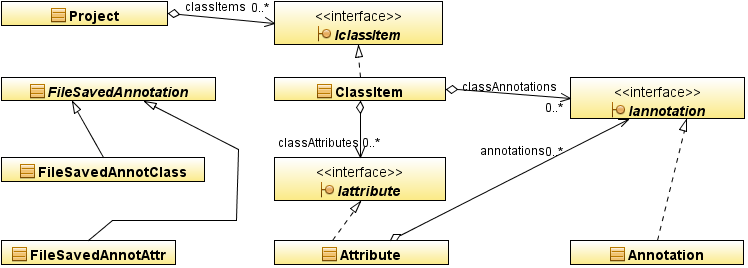
\includegraphics[scale=0.52]{Datova.png}
\caption{UML diagram datové vrstvy}
\end{center}
\end{figure}
\vspace{1.0cm}
Aplikační vrstva sestává z většího množství tříd, přičemž její oddělení od prezentační vrstvy je realizováno prostřednictvím rozhraní {\it IprojectManager}. Tento interface definuje všechny metody jak k úpravám jednotlivých anotací projektu, tak k samotnému vytváření, otevírání a ukládání projektu, včetně exportování anotovaných tříd. Třída {\it ProjectManager}, která toto rozhraní implementuje, obsahuje instanci třídy {\it Project}, nad kterou všechny deklarované metody operují, neboť nese všechna data projektu. Třída požadované operace neprovádí přímo, ale deleguje je na podřízené objekty, kterým předává případ-\\né parametry, a sama pak jejich prostřednictvím vrací požadovaná data nebo chybový kód v případě, že zachytí výjimku z některé nižší vrstvy. \\

Třída {\it ProjectLoader} zajišťuje vyváření nových a otevírání již existujících uložených projektů.
Vytvoření nového projektu poskytuje přetížená metoda {\it createProject}, která má v parametru buď cestu k JAR souboru nesoucímu všechny třídy, nebo list jednotlivých tříd. Druhým parametrem je název Java balíku, ve kterém byly všechny POJO třídy uložené. Jeho jméno je nezbytné pro pozdější načítání tříd reflexí.
V případě, že jsou třídy uložené v JAR archivu, dojde k jejich extrahování do dočasného adresáře prostřednictvím třídy {\it JarExtractor}, jejíž jediná veřejná metoda vrací list s jednotlivými dekomprimovanými třídami. Dále je voláním metod třídy {\it ProjectFilesCreator} vytvořen pracovní adresář aplikace včetně podadresáře dle názvu Java balíku POJO tříd, do kterého jsou všechny třídy nakopírovány, aby mohly být reflexí získány jejich atributy.


Z takto umístěných souborů je již možné získat všechna potřebná data ze kterých třída {\it ClassItemsGenerator} sestavuje list instancí datových tříd {\it ClassItem}, jež tato data ponesou. 
Anotace samotných tříd jsou vytvářeny třídou {\it ClassAnnotationCreator}, která volá metodu třídy {\it LoadAvailableAnnot}. Ta načítá seznam dostupných anotací pro třídy ze souboru, jehož název získává v parametru, a na základě jeho obsahu sestaví list instancí třídy {\it Annotation}, který také vrací. 
List atributů sestavuje třída {\it AttributeCreator}, která z cílové třídy načte pomocí reflexe seznam jejích atributů, na jejichž základě je vytvořen list instancí třídy {\it Attribute}. Každá tato instance obsahuje název atributu, který má zastupovat, a seznam anotací, který je sestaven opět metodou třídy {\it LoadAvailableAnnot}, tentokrát ale volanou s parametrem souboru nesoucím seznam dostupných anotací pro atributy.


Z listu instancí třídy {\it ClassItem} vytvoří {\it ProjectLoader} novou instanci třídy {\it Project}, která je navrácena do třídy {\it ProjectManager}. 
Všechny anotace v pro-\\jektu jsou po jeho vytvoření bez hodnot parametrů a příznaky nastaveny na hodnotu nepřidávat anotaci. Popisované vytváření projektu je také znázorněno UML diagramem na obrázku 5.2.

\begin{figure}[htb!]
\begin{center}
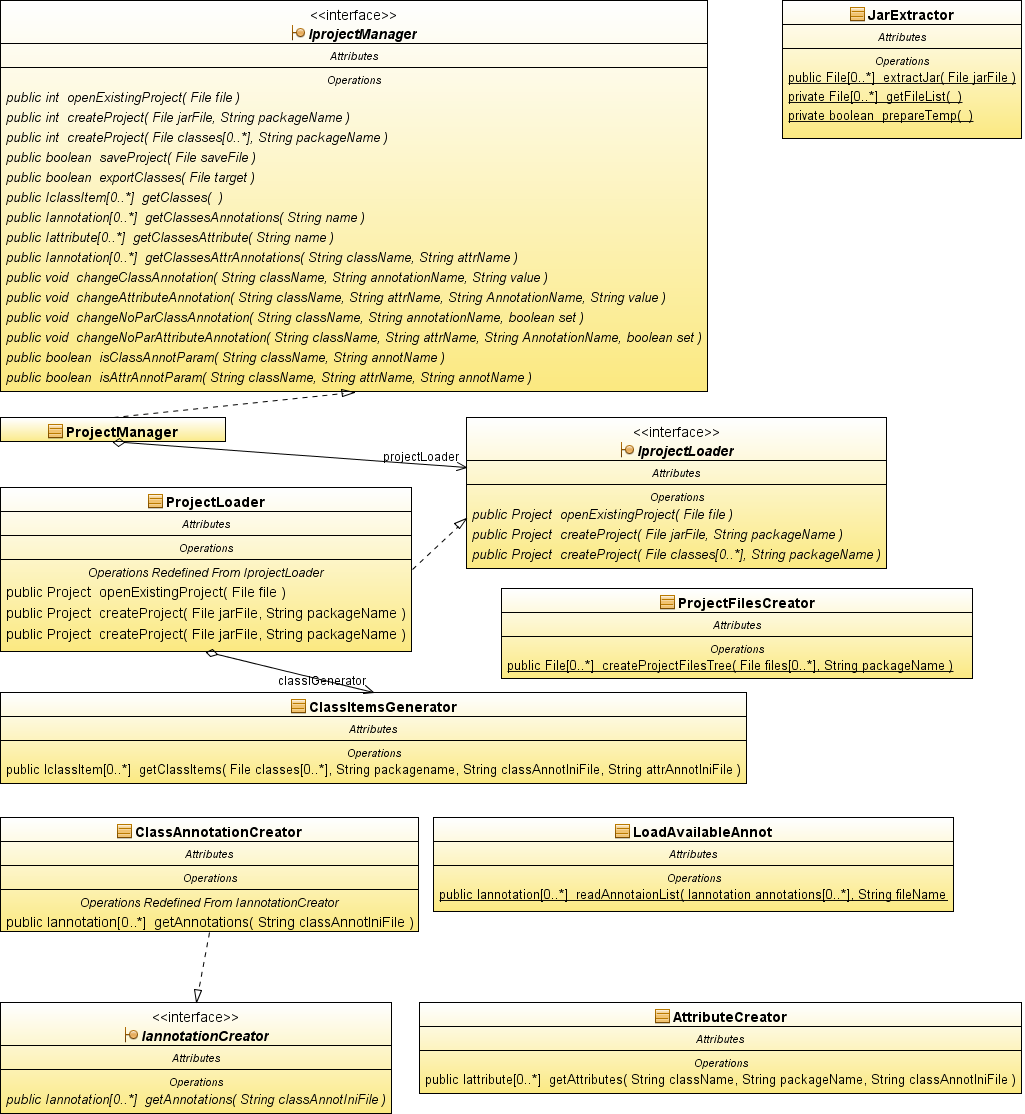
\includegraphics[scale=0.38]{Aplikacni1.png}
\caption{UML diagram tříd pro vytváření projektů}
\end{center}
\end{figure}


Otevírání uloženého projektu voláním metody {\it openExistingProject} probíhá podobně jako vytváření nového z JAR archivu. Uložený projekt je adresář komprimovaný do ZIP archivu, který nese přeložené POJO třídy a soubory {\it package.dat}, {\it annotations.dat}, {\it attrAnnots.ini} a {\it classAnnots.ini}. Poslední dva soubory obsahují seznamy přípustných anotací pro atributy a třídy, soubor {\it package.dat} obsahuje pouze název balíku POJO tříd a {\it annotations.dat} nese seznam uložených anotací.


Sestavení listu datových tříd {\it ClassItem} probíhá stejně jako při vytváření nového projektu, jen s tím rozdílem, že jméno Java balíku není získáno jako vstup prostřednictvím uživatele, ale je načteno ze souboru {\it package.dat} a při sestavování listu přípustných anotací jsou načítány příslušné soubory zároveň z kořenového adresáře aplikace, i z dočasné složky nesoucí extrahovaná data projektu. Třída {\it LoadAvailableAnnot} vytváří z načtených souborů dva listy přípustných anotací, které sloučí do jednoho, odstraní v něm opakující se prvky a vrací jej.


Načítání uložených anotací provádí třída {\it LoadedAnnotSetter}. Její jediná veřejná metoda nastavuje všechny příslušné anotace v listu tříd {\it ClassItem}, který získává parametrem společně se souborem uložených anotací. Ten je čtený třídou {\it SavedDataLoader}, která na jeho základě vytvoří list instancí potomků třídy {\it FileSavedAnnotation}, jež nesou jednotlivé uložené anotace. Tento list je pak sekvenčně čten a pro každou položku je nalezena v předchozím listu příslušná cílová anotace třídy či atributu, u které se nastaví získaná hodnota (v případě parametrické anotace), a příznak, že má být přidána. UML diagram na obrázku 5.3. znázorňuje třídy využité při otevírání projektu.
%\vspace{0.5cm}
\begin{figure}[htb!]
\begin{center}
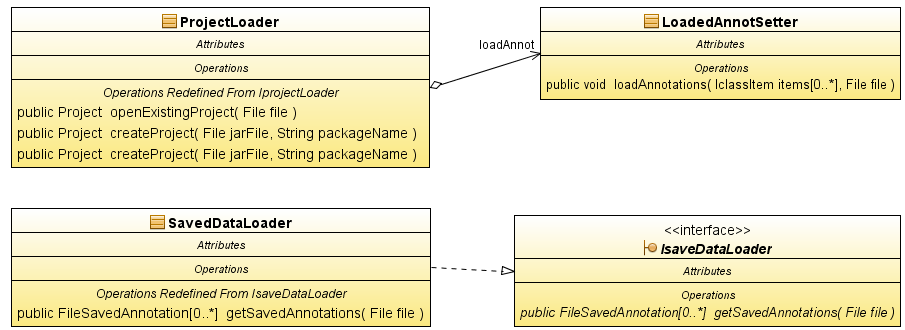
\includegraphics[scale=0.38]{Aplikacni2.png}
\caption{UML diagram tříd pro otevírání projektů}
\end{center}
\end{figure}\newline
Ukládání projektů zprostředkovává třída {\it ProjectSaver.} Ta využívá třídu {\it ChangeAnnotationsGather}, která z instance třídy {\it Project} získá všechny anota-\\ce označené jako přidávané k vytvoření listu instancí potomků třídy {\it FileSaved-\\Annotation}. Ten nese seznam anotací, který je potřeba uložit do souboru {\it annotations.dat}, což realizuje metoda {\it saveAnnotations} třídy {\it AnnotationData-\\Saver}. Dále je vytvořen soubor {\it package.dat}, do kterého je zapsán název Java balíku POJO tříd, jenž je uchováván ve třídě {\it Project}. Předchozí dva soubory jsou spolu s POJO třídami a soubory {\it attrAnnots.ini} a {\it classAnnots.ini} předány metodě {\it createJar} třídy {\it JarCreator}, která provede jejich zazipování do souboru na disk, jehož název volí uživatel.


Samotné modifikace POJO tříd dle vybraných anotací zajišťuje třída {\it ExportClasses}. Ta prostřednictvím třídy {\it ChangeAnnotationsGather} získá list instancí potomků třídy {\it FileSavedAnnotation}, který nese všechny požadované anotace. Z toho listu generují metody třídy {\it JaifFileGenerator} klíčový „jaif“ soubor, přičemž nezbytné konstantní řetězce získají ze třídy {\it Constants}. Z lis-\\tu požadovaných anotací je vytvořen seznam tříd, které je potřeba o tyto anotace doplnit. Dále je v pracovním adresáři aplikace vytvořen podadresář, do kterého se zkopírují všechny POJO třídy v původní podobě bez anotací. To realizuje třída {\it FileOperations}, která zároveň před každým provedením samotného anotování těmito soubory přepíše soubory v původním umístění. Díky tomu jsou vždy anotovány původní soubory, které tím pádem budou mít právě ty anotace, které uživatel vybral a žádné jiné (dodané předchozím anotováním). Samotné anotování pak probíhá cyklickým voláním hlavní metody knihovny {\it annotation-file-utilities.jar}, které jsou předány v parametru „jaif“ soubor a cílová POJO třída.


Po dokončení poslední iterace se všechny třídy projektu (včetně neanotova-\\ných) zkopírují do umístění zvoleného uživatelem, což zajišťuje opět třída {\it FileOperations} prostřednictvím svých statickým metod. Obrázek 5.4. obsahuje UML diagram tříd využívaných k ukládání projektu a exportování anotova-\\ných tříd. 

%\vspace{0.38cm}
\begin{figure}[htb!]
\begin{center}
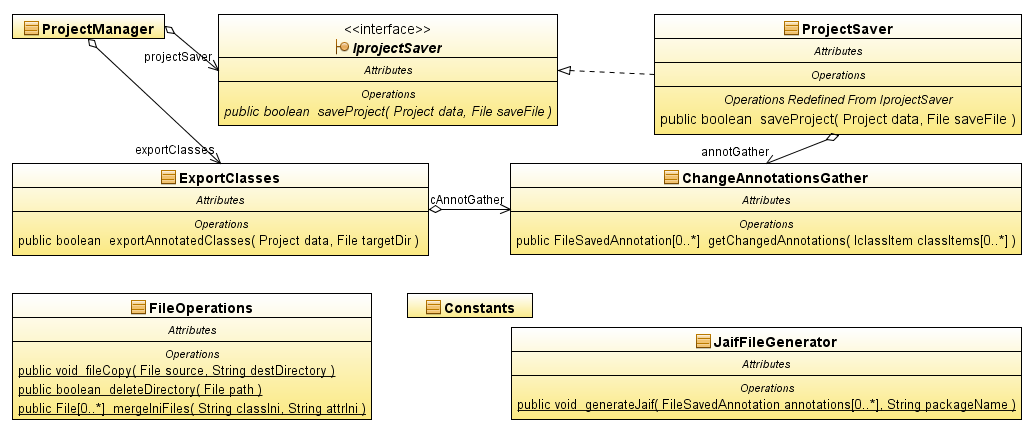
\includegraphics[scale=0.38]{Aplikacni3.png}
\caption{UML diagram tříd pro ukládání projektu a export dat}
\end{center}
\end{figure}


Veškerá nastavení a čtení hodnot anotací poskytuje třída {\it ProjectManager} voláním příslušných metod nad instancemi objektů datové vrsty.


Prezentační vrstva celé aplikace je realizována prostřednictvím knihoven AWT a Swing. 
Třída {\it MainWindow} slouží k zobrazení hlavního okna aplikace, které obsahuje základní menu. Na hlavním panelu okna se pak zobrazuje seznam atributů jednotlivých tříd včetně náhledu jejich anotací, který je ohraničen listem nesoucím název třídy. Třída {\it MainWindow} zároveň nese instanci třídy {\it Project}, jež předává dalším třídám posluchačů položek menu, které slouží k ukládání, otevírání a vytváření nových projektů, jejichž data zároveň zobrazují.


Třída {\it NewProjectListener} zajišťuje vytvoření nového projektu při vzniku požadavku prostřednictvím příslušné položky menu. V prvním kroku se zobrazí dotazovací okno, zda budou zpracovávané třídy vybrány jednotlivě nebo zabalené do JAR archivu. Tento archiv, respektive jednotlivé soubory jsou pak vybrány v následujícím okně. V posledním okně se zadá název Java balíku importovaných tříd. Všechna získaná data jsou předána volané metodě {\it createProject} instance třídy {\it Project}. Pokud dojde při vytváření nového projektu k nějaké chybě, je zobrazena odpovídající chybová hláška. V opačném případě se z vytvořeného projektu získají všechna data, která je potřeba zobrazit. To zajišťuje třída {\it DisplayProjectData}, která vytváří listy se seznamy atributů tříd, jejíž názvy jsou obsaženy v záhlaví každého listu. Zároveň je vytvořen jeden list nesoucí názvy všech tříd. Každý vytvořený list ještě obsahuje kromě seznamu atributů třídy, respektive názvů všech tříd, také náhled nastavených anotací u vybraného atributu, resp. třídy. Celý seznam je zobrazen jako tabulka {\it JTable} knihovny Swing, jejíž položky jsou obsaženy v datovém modelu třídy {\it JTableDataModel}. Při výběru více položek tabulky jsou v náhledu zobrazeny jen ty anotace, které jsou pro vybrané položky shodné, což testují metody třídy {\it CommonAnnots}. Tlačítko zobrazené pod náhledem slouží ke změně anotací všech vybraných položek, což zajišťuje třída {\it DisplayAnnotations}, volaná prostřednictvím třídy {\it ButtonChGroupListener} posluchače tlačítka.


Třída {\it DisplayAnnotations} zobrazuje nové okno, které obsahuje seznam názvů všech dostupných anotací pro vybrané atributy, resp. třídy. Pro každou anotaci je zobrazeno zaškrtávací políčko rozhodující, zda má být přidána, a v případě parametrické anotace také textové pole pro zadání hodnoty parametru. Dvě tlačítka v zápatí okna slouží pro uložení nebo zrušení změn. Při stisku tlačítka zrušení změn je okno pouze zavřeno. Při stisku tlačítka uložení změn se cyklicky otestují stavy všech zaškrtávacích políček a dle jejich hodnot se v datech projektu nastaví hodnoty příznaků anotací pro přidání respektive i hodnoty parametrů získané z odpovídajících textových polí v pří-\\padě parametrických anotací.


Třída {\it OpenProjectListener} umožňuje otevření již existujícího uloženého projektu při uživatelském výběru položky menu hlavního okna. Při obsluze tohoto požadavku se zobrazí okno pro výběr souboru uloženého projektu. Cesta k tomuto souboru je předána jako parametr volané metodě {\it openExisting-\\Project} instance třídy {\it Project}. Pokud není soubor poškozený, což by způsobilo vyvolání okna s chybovou hláškou, dojde k zobrazení veškerých dat stejným způsobem jako při vytváření nového projektu.


Ukládání otevřeného či nově vytvořeného projektu zajišťuje třída {\it SaveAs-\\ProjectListener}, která zobrazuje okno pro výběr umístění a názvu ukládaného projektu. Získanou hodnotu pak předává volané metodě {\it saveProject} instance třídy {\it Project}, která samotné uložení provede.
Přidání anotací a export anoto-\\vaných tříd je zajištěn prostřednictvím třídy {\it ExportClassesListener} sloužící jako posluchač příslušného tlačítka menu, která zobrazí okno pro výběr umístění anotovaných tříd. Tuto hodnotu pak předá jako parametr metodě {\it exportClasses} instance třídy {\it Project}, jež provede samotné anotování tříd a je-\\jich uložení do vybraného místa.


Podrobnější detaily o aplikaci jsou pak patrné ze zdrojových kódů progra-\\mu, respektive z připojených podrobných Javadoc komentářů a z kompletního UML diagramu v příloze B.
Postup při ovládání aplikace popisuje uživatelská dokumentace dostupná v příloze A.


\chapter{Testování}
\hspace{0.65cm}V rámci této práce byla aplikace Annotation Tool navrhnuta a od základu implementována, proto je nutné provést její otestování. Pro datovou a apli-\\kační vrstvu programu byly z důvodu jednoduchosti vybrány testy JUnit, které umožňují prověřit funkčnost jednotlivých komponent. V Datové vrstvě byly vytvořeny testy pro každou třídu s výjimkou abstraktní třídy {\it FileSaved-\\Annotation}, neboť ta je již testována prostřednictvím testů svých potomků. 
Pro aplikační vrstvu byly rovněž vytvořeny testy pro všechny třídy, s výjimkou třídy {\it Constants}, která obsahuje pouze veřejné statické konstanty, které nemá smysl testovat. 
Každý test slouží k testování veřejných metod a konstruktorů právě jedné třídy, podle níž je zároveň pojmenován. Vzhledem k tomu, že aplikace byla v průběhu vývoje průběžně testována metodou ladících výpisů, vytvořené testy odhalily jen několik drobných chyb, které byly následně opraveny. Testy při spuštění nad poslední verzí aplikace tedy probíhají se 100\% úspěšností, což bylo také cílem.

V prezentační vrstvě aplikace JUnit testy vytvořeny nebyly, protože většina metod těchto tříd vrací nebo získává v parametrech objekty knihovny Swing, které by se tímto způsobem testovaly velmi obtížně. Z toho důvodu a ve snaze o zachycení co nejvíce chyb bylo ještě provedeno otestování běhu aplikace při zpracovávání reálných dat. Z relační databáze Portálu byly nástrojem Hibernate Tools vygenerovány a následně přeloženy POJO třídy, které slouží jako reprezentativní vstupní data.Ta byla následně importována do nového projektu, který byl opakovaně otevírán, pozměněn a opět uložen. V každé iteraci byly vyexportovány anotované třídy a následně otevřeny Class File Editorem ve vývojovém prostředí Eclipse, kde byla provedena ruční kontrola každé třídy, zda obsahuje právě ty anotace, které byly uživatelem v nástroji nastavené. Zároveň proběhla kontrola, zda se při opětovném otevření projektu zobrazí právě ty změny, které byly při jeho poslední úpravě uloženy. Tyto testy byly prováděny už při samotném vývoji aplikace a odhalily několik středně závažných chyb, které byly následně opraveny. Provedení těchto testů nad finální verzí programu už žádné chyby neodhalilo.


Díky výše uvedeným testům se podařilo úspěšně odladit stabilní, korektně pracující verzi aplikace, kterou je možné efektivně využívat k požadovanému účelu.


\chapter{Závěr}
\hspace{0.65cm}Z první části práce, která se zabývala možnostmi reprezentace dat v pro-\\středcích sémantického webu, plyne, že pro uchování dat portálové databáze je nejvhodnější zápis ve formátu OWL. Tento jazyk poskytuje dostatečné vyjadřovací možnosti a dovoluje zapisovat i sémantiku, kterou je požadováno datům dodávat.


Z další části, která se zabývá samotnou transformací, plyne, že nejvhod-\\nějším způsobem převodu dat je vytvoření objektového datového modelu z portálové databáze v podobě POJO objektů prostřednictvím frameworku Hibernate, které slouží jako vstup nástroje Jenabean.  
Požadovaná data ve formátu OWL poté vygeneruje nástroj OWL API, jehož vstupem je právě výstup aplikace Jenabean.


Nástroj Jenabean zároveň dovoluje dodávat datům sémantiku prostřed-\\nictvím Java anotací nad elementy vstupních POJO objektů. V rámci této práce byly v nástroji opraveny nefunkční anotace a také implementovány nové, které dovolují dodávat další sémantiku, již jazyk OWL umožňuje zapsat. Opakovanou kontrolou výstupu transformace při použití anotací v POJO třídách se prokázalo, že úpravy nástroje byly provedeny úspěšně, a to i přes absenci jeho programátorské dokumentace.


Aby nebylo nutné ručně přidávat anotace jednotlivým POJO třídám a následně je překládat, 
byl vytvořen nástroj, který tento problém řeší. Navrhnutá a implementovaná aplikace Annotation Tool umožňuje přidávat přeloženým POJO třídám vybrané anotace jednoduše prostřednictvím grafic-\\kého uživatelského rozhraní.
Poslední část práce, která se zabývá testováním vytvořeného nástroje, prokázala jeho správnou funkčnost, a problém přidání sémantických informací se tak jeví jako úspěšně vyřešený.


Práci lze považovat za úspěšnou, neboť se podařilo navrhnout automatic-\\kou transformaci dat z EEG/ERP portálu do formátu OWL a to včetně možnosti jednoduchého přidávání sémantických informací výsledným datům. V práci by bylo možné dále pokračovat v implementaci dalších anotací do nátroje Jenabean či upravovat aplikaci Annotation Tool tak, aby byla schopna pracovat i se složitějšími typy anotací.



%\section{EEG}
%\subsection{EEGecko}
\newpage
\thispagestyle{plain}
\noindent
{\bf \LARGE Seznam zkratek a pojmů}\\
%\addcontentsline{toc}{chapter}{Seznam zkratek a pojmů}

\noindent
\begin{description}
\item[API] Application Programming Interface, rozhraní pro programování aplikací
\item[AWT] Abstract Window Toolkit, knihovna Javy pro tvorbu grafického uživa-\\telského rozhraní
\item[EEG] Electroencephalography, metoda vyšetření elektrické aktivity centrál-\\ního nervového
systému
\item[ERP] Event Related Potential, vyšetření reakcí mozku na vnější podněty
\item[JAR] Java Archive, archivní soubor Javy založený na ZIP kompresi
\item[NIF] Neuroscience Information Framework, webové úložiště neuroinformatic-\\kých dat a experimentů
\item[OWL] Web Ontology Language, ontologický jazyk sémantického webu
\item[POJO] Plain Old Java Object, třída jednoduchého objektu jazyka Java
\item[RDF] Resource Description Framework, metodika modelování informací \\v sémantickém webu
\item[SPARQL] SPARQL Protocol and RDF Query Language, dotazovací jazyk nad RDF grafy
\item[URI] Uniform Resource Identifier, jednotný identifikátor zdroje informací
\item[W3C] World Wide Web Consortium, organizace vyvíjející webové standardy
\item[XML] Extensible Markup Language, značkovací jazyk vyvinutý W3C
\item[XSD] XML Schema Definition, XML schéma popisující strukturu XML doku-\\mentu
\item[ZIP] souborový formát sloužící ke komprimování a archivaci dat.
\end{description}



%\bibliographystyle{alpha}
%\bibliographystyle{csplainnat}
\bibliography{bakalarka}
\bibliographystyle{plain}
%\addcontentsline{toc}{chapter}{Literatura}


\appendix
\newpage
% Konec cislovani

\thispagestyle{plain}

\noindent
{\bf \LARGE Přílohy}
\setcounter{chapter}{1}

\newpage
\thispagestyle{plain}
\section*{{\LARGE A} Uživatelská dokumentace}
\hspace{0.65cm}Aplikace Annotation Tool je nástroj sloužící k dodávání Java anotací zkompilovaným POJO třídám. Pro sestavení a spuštění nástroje je zapotřebí Java JDK verze 6.0 či vyšší a nástroj Ant. Kořenový adresář se zdrojovými soubory obsahuje soubor {\it build.xml}, což umožňuje přeložit a sestavit program v příkazovém interpretu příkazem {\it ant}. Sestavením vznikne spustitelný soubor {\it AnnotationTool.jar} a dva konfigurační sobory s příponou {\it ini}. V souboru
{\it classAnnots.ini} je zapsán seznam všech anotací dostupných pouze pro třídy. Každý řádek představuje jednu anotaci, přičemž musí začínat znakem {\it P} pro parametrickou anotaci nebo znakem {\it N} pro neparametrickou anotaci. Za ním následuje znak {\it @}, po kterém se uvede název anotace. Soubor {\it attrAnnots.ini}, jež má stejný formát zápisu, definuje seznam dostupných anotací jen pro atributy tříd. Modifikací těchto souborů se docílí změny seznamu anotací, které bude anotační nástroj uživateli nabízet.

Program se spouští v grafickém prostředí operačního systému spuštěním souboru {\it AnnotationTool.jar} nebo z příkazového interpretu příkazem {\it java –jar AnnotationTool.jar}. 
Po spuštění aplikace se zobrazí okno, které obsahuje menu s nabídkami {\it Project} a {\it Annotation}. 
Položka {\it NewProject} nabídky {\it Project} slouží k vytvoření nového projektu. Uživatel je vyzván, zda chce do projektu POJO třídy importovat jednotlivě nebo zabalené do JAR archivu. V dalším okně se provede výběr požadovaných POJO tříd nebo JAR archivu v závislosti na předchozí volbě. V posledním zobrazeném okně se zadá název Java balíku, do kterého všechny importované třídy náleží. Pokud je struktura názvů balíků stromová, oddělují se názvy znakem „.“.


Položka {\it OpenProject} nabídky {\it Project} slouží k otevření uloženého projektu, který uživatel vybere prostřednictvím zobrazeného okna pro výběr souboru. 
Po vytvoření nového či otevření existujícího projektu se v hlavním okně aplikace (viz obrázek A.1) zobrazí seznam listů, který je přepínatelný v horní části okna, kde jsou uvedeny jejich názvy. Každý list, jehož název odpovídá jménu třídy, obsahuje seznam, jehož první položkou je jméno třídy a za ní následuje seznam všech jejích atributů. Výběrem položky seznamu se v pravé části okna zobrazí seznam jejích vybraných anotací, který je možné změnit tlačítkem {\it Change selected}. Pokud je v seznamu vybráno více položek, jsou v náhledu zobrazeny jen ty anotace, které mají vybrané položky společné. Tlačítkem {\it ChangeSelected} se pak mění anotace společně všem vybraným položkám najednou.\\

\begin{figure}[htb!]
\begin{center}
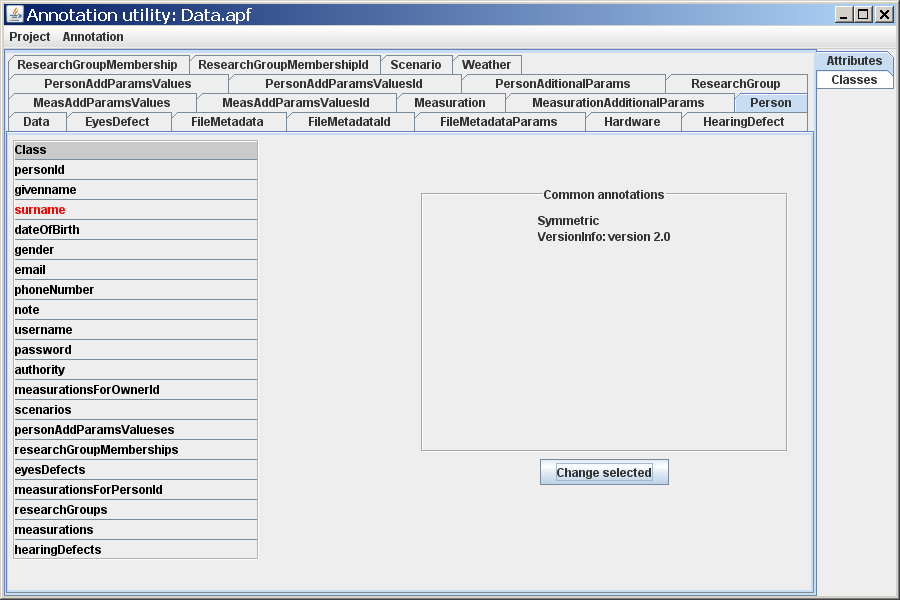
\includegraphics[scale=0.5]{Hlavni.png}
\caption{Hlavní okno aplikace}
\end{center}
\end{figure}


Při požadavku změny anotací se zobrazí nové okno (viz obrázek A.2), které obsahuje seznam všech dostupných anotací pro dané položky. Vedle každého názvu anotace je zobrazeno zaškrtávací políčko pro označení, zda má být anotace přidána, a pokud se jedná o parametrickou anotaci, je vedle něj uvedeno textové pole, do kterého se tato hodnota zadává. Uložení změn se provede tlačítkem {\it Save} a jejich zrušení tlačítkem {\it Cancel} ve spodní části tohoto okna.

\vspace{0.1cm}
\begin{figure}[htb!]
\begin{center}
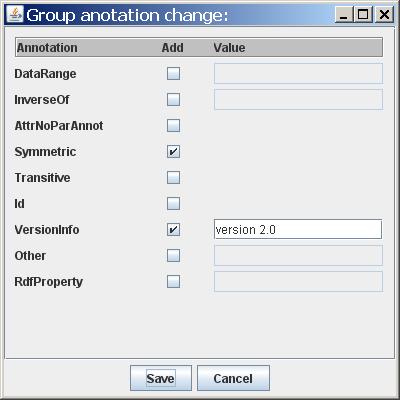
\includegraphics[scale=0.5]{Nastav.png}
\caption{Okno pro změnu anotací}
\end{center}
\end{figure}

\thispagestyle{plain}

V pravém horním rohu hlavního okna jsou umístěny ještě dvě záložky. První s názvem {\it Attributes} zobrazuje výše popsané listy, druhá záložka {\it Classes} přepíná na list, nesoucí seznam všech tříd, který slouží ke hromadné změně anotací tříd samotných. 
Uložení vytvořeného projektu na disk je možné skrze položku {\it Save as} nabíky {\it Project}, kdy je uživatel vyzván k výběru umístění a zadání názvu projektu. Položka {\it Save} slouží pouze k uložení provedených změn v již uloženém projektu.


K exportování anotovaných tříd slouží položka {\it Annotate Class files} nabídky {\it Annotation}. Při tomto požadavku je uživatel vyzván k výběru adresáře, do kterého budou soubory umístěny.

\thispagestyle{plain}

\newpage
\thispagestyle{plain}
\section*{{\LARGE B} UML diagram aplikace Annotation Tool}
- viz následující list formátu A3

\newpage
\thispagestyle{empty}

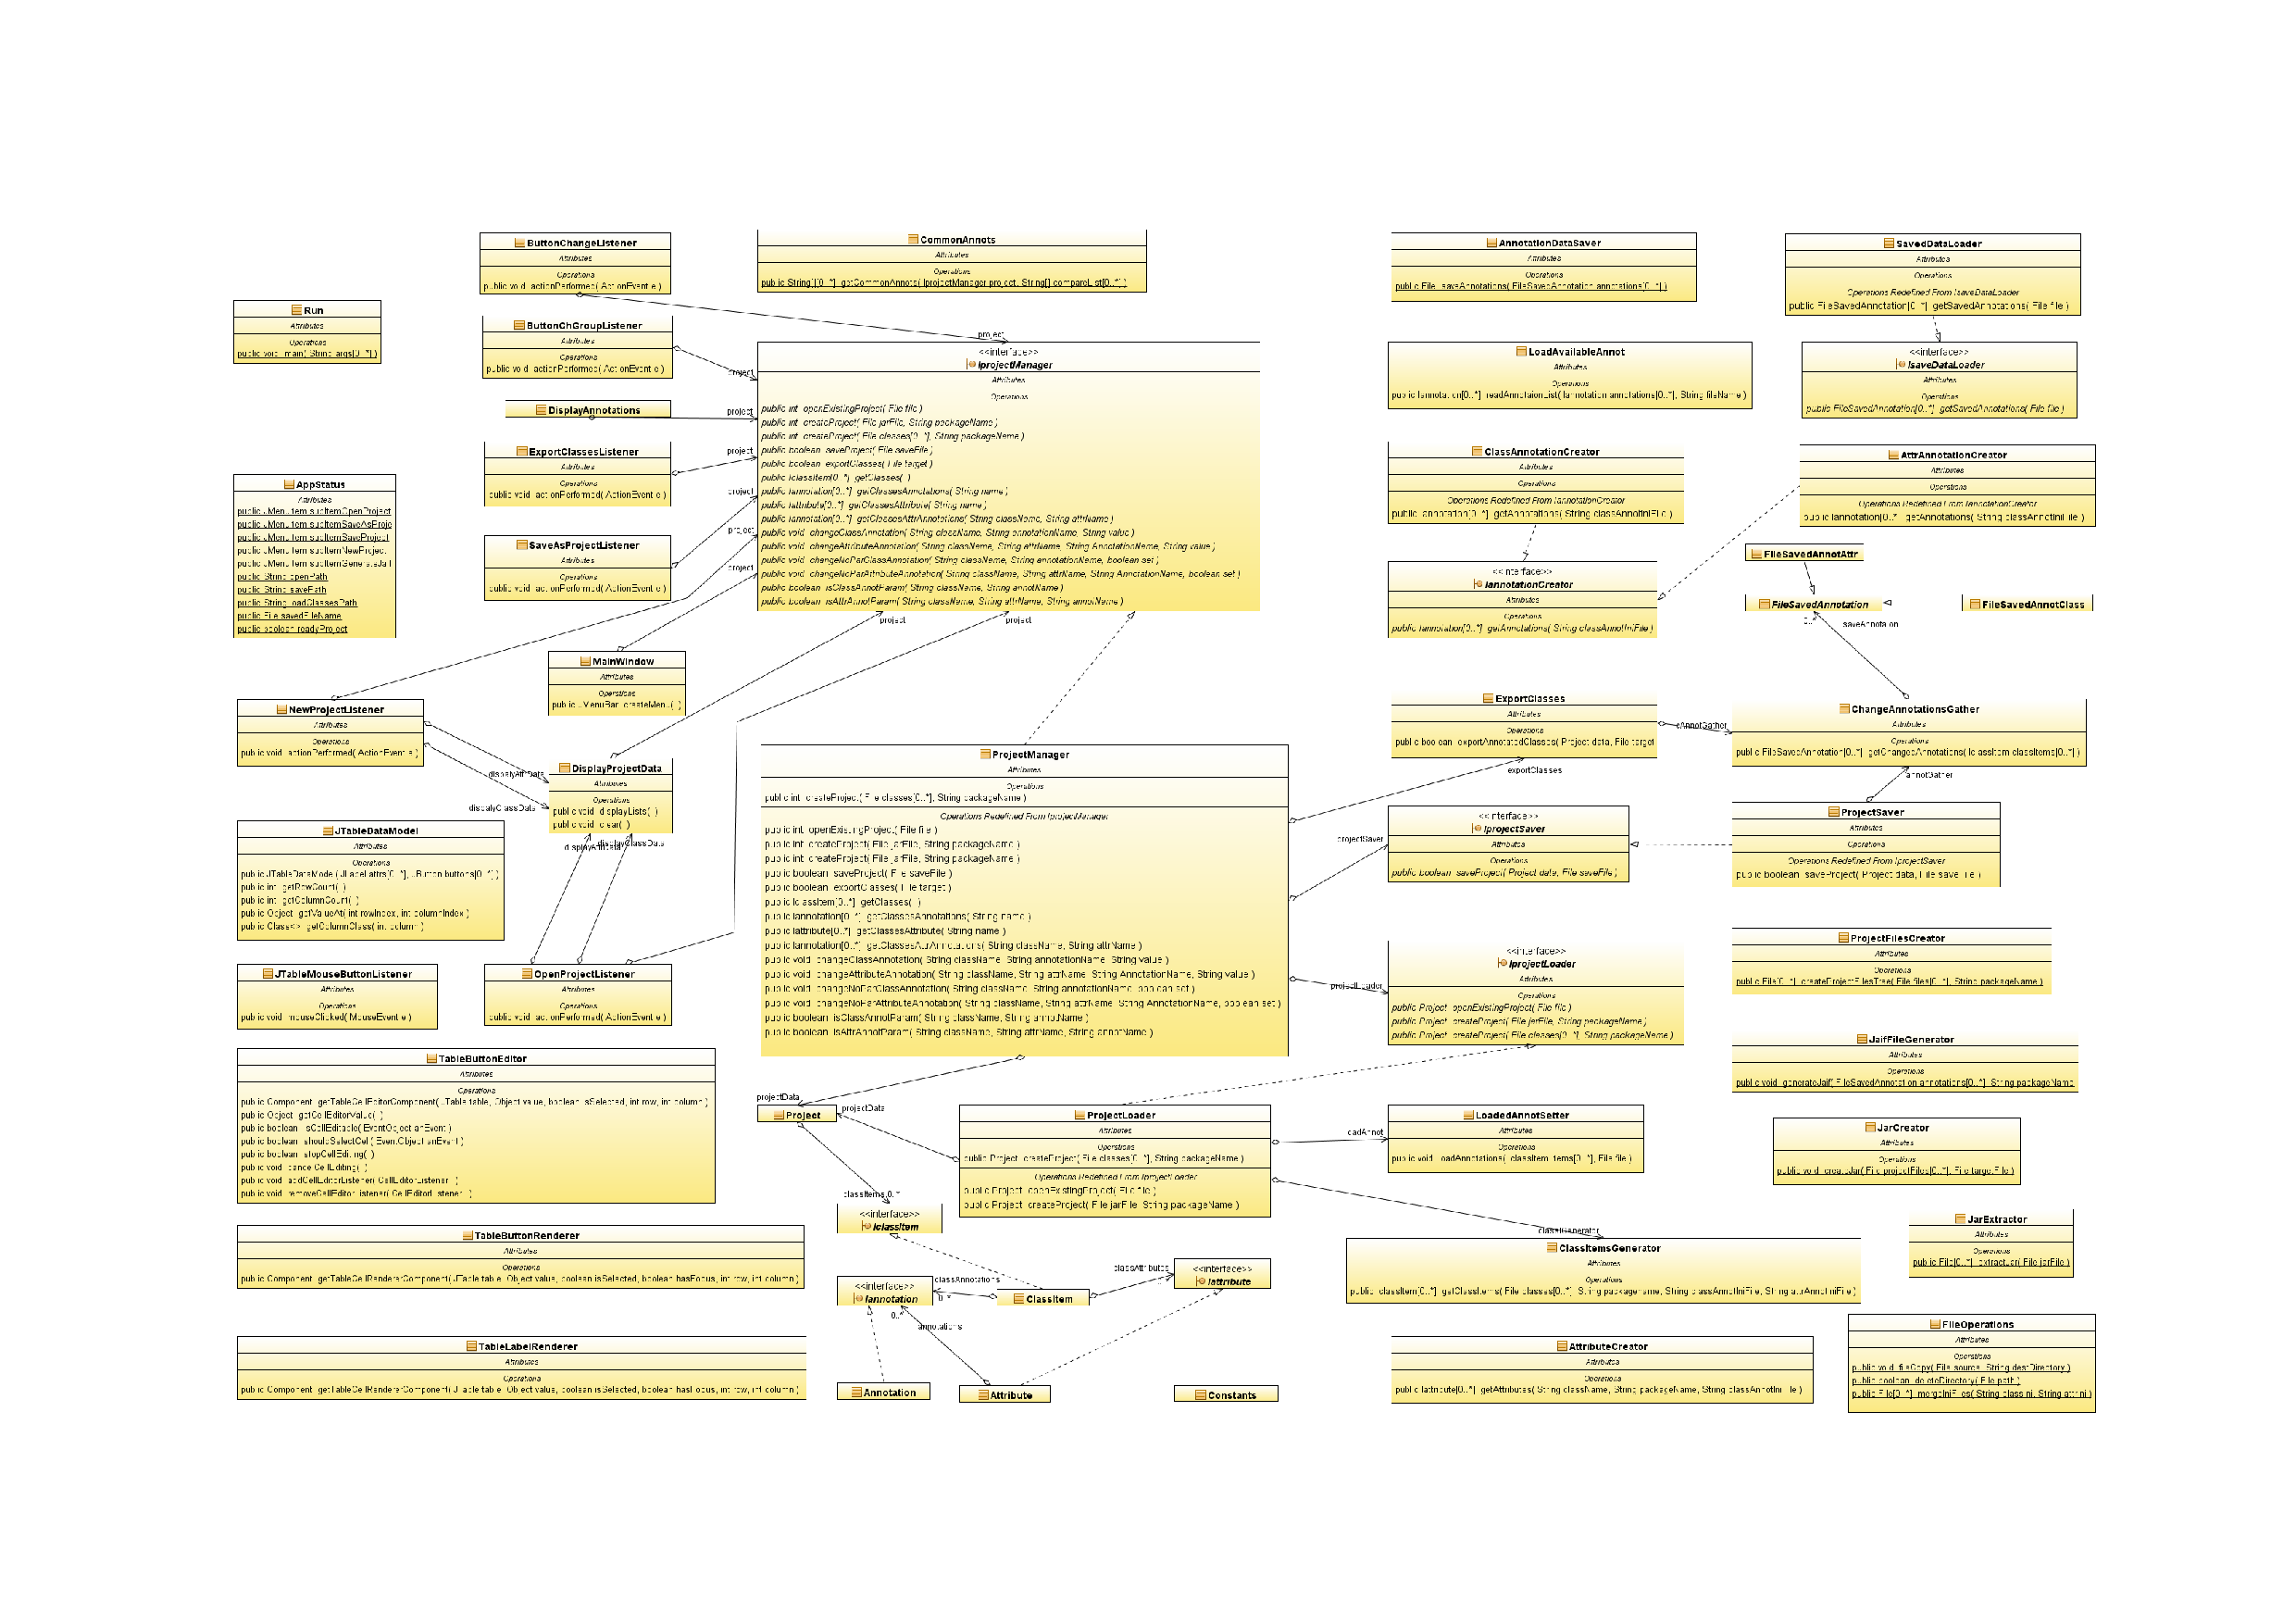
\includepdf[angle=270]{umlAll.pdf}


\end{document}
